\chapter{Grundlagen}\label{kap:Grundlagen}
\newpage
\section{Softcore-Prozessoren}\label{kap:softcoreprozessoren}

Ein Soft Core (engl. „Software-Kern“) ist ein Prozessor, Mikrocontroller oder ein Signalprozessor, welcher als virtuelle Einheit in einem \ac{fpga} oder \ac{asic} integriert wird.
Dies bietet die Möglichkeit einem digitales Schaltungsdesign jeden beliebigen Prozessor hinzuzufügen. Umgesetzt wird dieser Vorgang im \ac{fpga} durch reine Anwenderlogik,
welche dementsprechend konfiguriert werden muss.\\
Das typische Anwendungsgebiet eines SoftCores ist die Lösung von komplizierten Aufgaben, mit denen klassische „State Machines“ überfordert sind oder die Effektivität
 nicht mehr gegeben ist. Somit werden Softcores oftmals nachträglich in bestehende Designs eingefügt, wenn deren Umfang sich extrem vergrößert hat.\\

\subsection{Vergleich SoftCores und HardCores}\label{kap:vergleich}
Vorteile:
\begin{itemize}
   \item Flexible Anwendung: Das \ac{fpga} kann bei Bedarf mit einem SoftCore versehen werden, jedoch wird nicht von vorneherein Platz für einen HardCore verschwendet, welcher
    dann letztendlich ungenutzt bleibt. Daraus ergeben sich deutliche Vorteile im Hinblick auf die Kosten.
    \item Konfigurierbarkeit: Beim Softcore deutlich flexibler, da hier unter anderem die Größe der Datenpfade und die Anzahl der Zusatzmodule variiert werden kann.
 \end{itemize}


Nachteile:
\begin{itemize}
  \item SoftCores haben auf Grund ihrer Flexibilität einen deutlichen Geschwindigkeitsnachteil
\end{itemize}

\subsection{Typen}\label{kap:typen}
Es gibt eine große Anzahl verschiedener SoftCores. Diese unterscheiden sich aber maßgeblich in der Größe der Datenpfade.
Somit wird unterschieden zwischen 8-,16- und 32-Bit Systemen.\cite{softcore}\\


\section{Memory Management Unit}\label{kap:mmu}

Bei der \ac{mmu} handelt es sich um einen so genannten Coprozessor, welcher die Speicherverwaltung des Arbeitsspeichers übernimmt. Umgesetzt wird diese Verwaltung mit
Hilfe von Paging, welches virtuelle Adressen auf physikalische Adressen abbildet. Der gesamte Speicher wird in einzelne Speicherbereiche unterteilt und dann von der
\ac{mmu} den jeweiligen Prozessen zugeteilt. Ebenfalls überwacht Sie die Einhaltung dieser Bereiche und unterbricht gegebenenfalls Instruktionen, die auf einen verbotenen
Bereich zugreifen wollen.\cite{itwissen}\\

\begin{figure}[H]
\centering
\includegraphics[width=0.8\textwidth]{Hauptteil/mmu.eps}
\caption{Blockschaltbild einer MMU}\label{fig:mmu}
\end{figure}

\section{Interrupt}\label{kap:interrupt}
Neben der \ac{cpu} und dem Datenspeicher haben die meisten Computersysteme Peripherie. Es handelt sich dabei um verbaute oder um an Schnittstellen angeschlossene Geräte.
Damit die \ac{cpu} die Nachricht erhält, dass Daten an solch einer Schnittstelle beziehungsweise Verbindung anliegen, muss es eine Möglichkeit geben den Prozessor zu
unterbrechen. Hier gibt es die Art des sogenannten Polling, bei dem der Prozessor alle vorhandenen Eingabegeräte zyklisch abfragt. Ein effektiveres Verfahren ist die
Unterbrechungsanforderung (Interrupt), welche eintritt, wenn Daten anliegen. \\
Sobald ein Gerät Daten zur Weiterverarbeitung besitzt, wird ein \ac{irq} auf der dafür vorgesehenen Interrupt-Leitung gesendet. Daraufhin unterbricht der Prozessor
seine Arbeit und verarbeitet die Daten des Gerätes.\\

\begin{figure}[H]
\centering
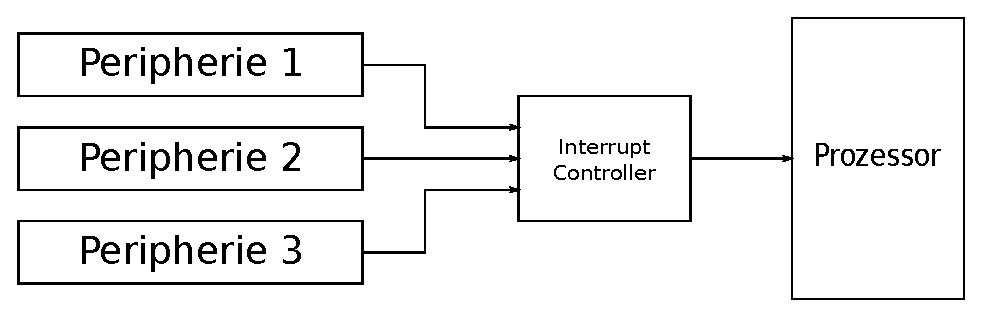
\includegraphics[width=0.8\textwidth]{Hauptteil/irq.eps}
\caption{Interrupt-Controller}\label{fig:irq}
\end{figure}


 \section{Peripherie}\label{kap:peripherie}
 Ein Peripheriegerät kann einer Hardware hinzugefügt werden um die Fähigkeiten zu erweitern. Sie sind optional im Gegensatz zu der Hardware, welche in den vorherigen
 Kapiteln beschrieben wurde.

\subsection{UART}\label{kap:uart}

Um mit Peripheriegeräten zu kommunizieren, kann \ac{uart} als serielle Schnittstelle genutzt.
Bei dieser Art der Kommunikation werden serielle Daten zwischen dem Board (\emph{Master})
und dem Empfänger (\emph{Slave}) ausgetauscht. Dabei spielen die TxD und die RxD-Datenleitungen
eine wichtige Rolle, da der Datenaustausch über diese Leitungen realisiert wird.\\
Im Gegensatz zu der \ac{spi}-Schnittstelle (~\ref{kap:spi}), wird kein Clock-Signal
übertragen um Daten zu validieren. Des Weiteren wird die Verbindung mit einer definierten
Geschwindigkeit realisiert, der sogenannten \emph{Baudrate}. \cite{uartpdf} \\
Die Baudrate bezeichnet dabei die Anzahl der Bits, welche pro Sekunde übertragen werden.
\ac{uart} konvertiert die Bytes in serielle Bits, überträgt diese über eine einzelne Leitung
und liest die zugehörigen Start- und Stop-Bits aus.\\
Das sogenannte \emph{Character}(Zeichen) besteht aus einer konfigurierbaren Anzahl an Datenbits (in den meisten
Fällen 7 oder 8), aus einem \emph{low-level} Start-Bit , einem optionalen Parity-Bit und einem
oder mehreren logischen \emph{high-level} Stop-Bits.\\
Das Start-Bit teilt dem Receiver mit, dass ein neues \emph{Character} empfangen wird.
Die nächsten Bits, je nachdem wie viele Daten-Bits vorher konfiguriert wurden , stellen
dann den Inhalt des \emph{Character} dar. Darauf folgt das optionale Parity-Bit,
welches anzeigt, ob die Anzahl der mit '\emph{1}' belegten Daten-Bits gerade oder
ungerade ist. Am Ende der Folge stehen dann entweder ein oder zwei  \emph{high-level } Stop-Bits,
welche dem Receiver eindeutig signalisieren, dass die Übertragung vollständig ist. Dadurch,
dass das Start-Bit \emph{high-level} (1) und das Stop-Bit \emph{low-level} (0) ist,
ist immer eine klare Abgrenzung zwischen dem derzeitigen und dem folgenden \emph{Character} möglich.\\

Die Datenübertragung lässt sich nach~\ref{fig:uart} darstellen.\\

\begin{figure}[h!]
\centering
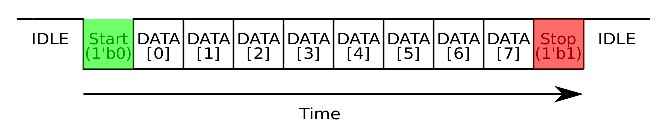
\includegraphics[width=0.8\textwidth]{Hauptteil/uart.eps}
\caption{Datenübertragung per \ac{uart} }
\label{fig:uart}
\end{figure}







\chapter{Soft Cores}\label{kap:softcores}
\newpage
\section{MicroBlaze}\label{kap:microblaze}



\subsection{Erstellen der Hardwarekonfiguration}\label{kap:microblazehardware}


Schritt 1:
Starten Sie Vivado und wählen Sie „New Project“ aus.
Hierbei wählt man „RTL Project“ als Projekttyp, wobei der Haken bei „ Do not specify sources at this time“ gesetzt sein sollte.\\

Schritt 2:
Nun gilt es unter dem Tab „Boards“ das korrekte Board auszuwählen, in meinem Fall war es das Nexys4 DDR.
Anschließend klicken Sie auf „Finish“ und das Projekt wird erstellt.\\


Schritt3:

Im Flow Navigator  auf der linken Seite wählt man nun „Create Block Design“ aus und
 gibt diesem Design einen beliebigen Namen.
Es öffnet sich das Block Design, bei dem der Tab „Board“ zu wählen ist. Hier werden nun
alle Bausteine für das Nexys4 DDR-Board angezeigt.\\

\begin{figure}[H]
\centering
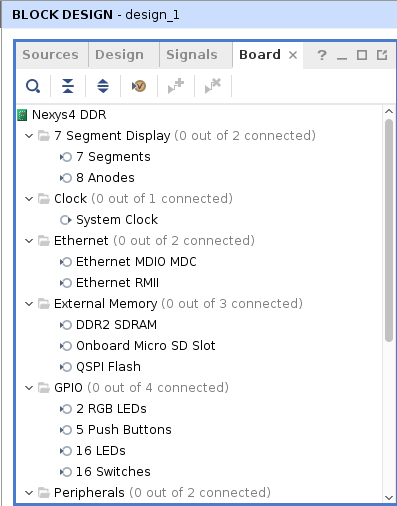
\includegraphics[width=0.8\textwidth]{Hauptteil/schritt3.png}
\caption{IP Integrator Block Design Diagram}\label{fig:mbschritt3}
\end{figure}

Schritt 4:

Durch doppeltes Klicken auf die Bausteine werden zunächst die „System Clock“, „USB UART“ und „DDR2 SDRAM“ hinzugefügt. Die folgenden Fenster werden jeweils mit OK bestätigt.
Im Design Diagram kann nun über das „+“-Symbol der Microblaze und der „AXI Timer“ eingefügt werden.\\


Schritt 5:


Der „Clocking Wizard“ muss wie im folgenden Bild konfiguriert werden.

\begin{figure}[H]
\centering
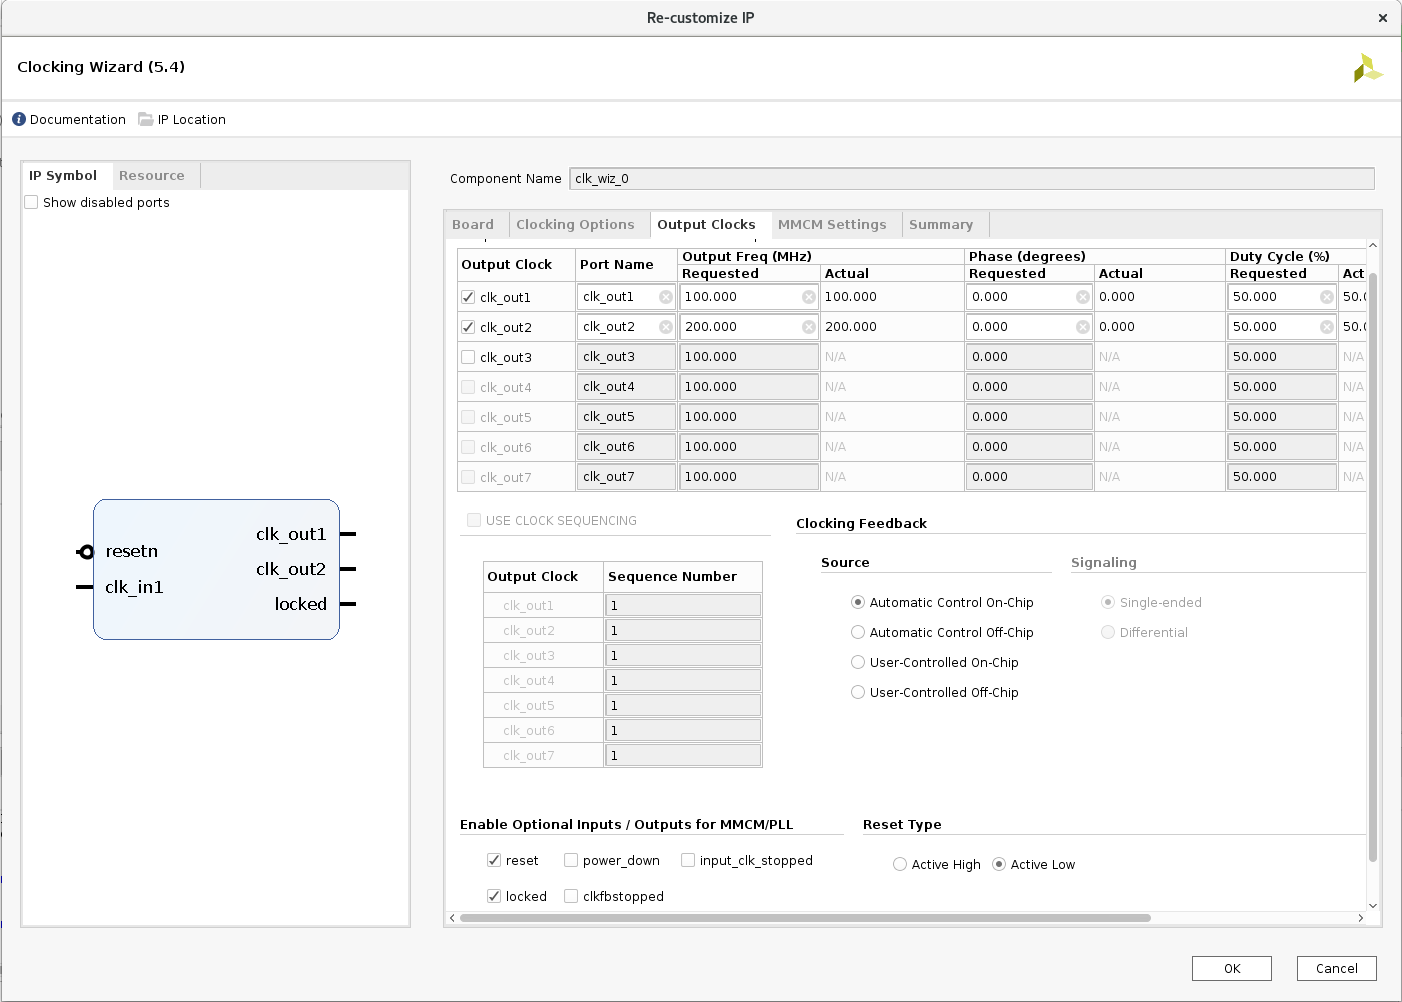
\includegraphics[width=0.8\textwidth]{Hauptteil/Schritt5.png}
\caption{Einstellungen des Clocking Wizard}\label{fig:mbschritt5}
\end{figure}

Dabei wird eine zweite Output Clock auf 200MHz gesetzt, sowie der Reset Type auf „Active Low“.


Schritt 6:

Die bestehende Verbindung zwischen der SysClock und dem MIG muss gelöscht werden und eine neue zwischen dem Clocking Wizard und dem MIG erstellt werden.

\begin{figure}[H]
\centering
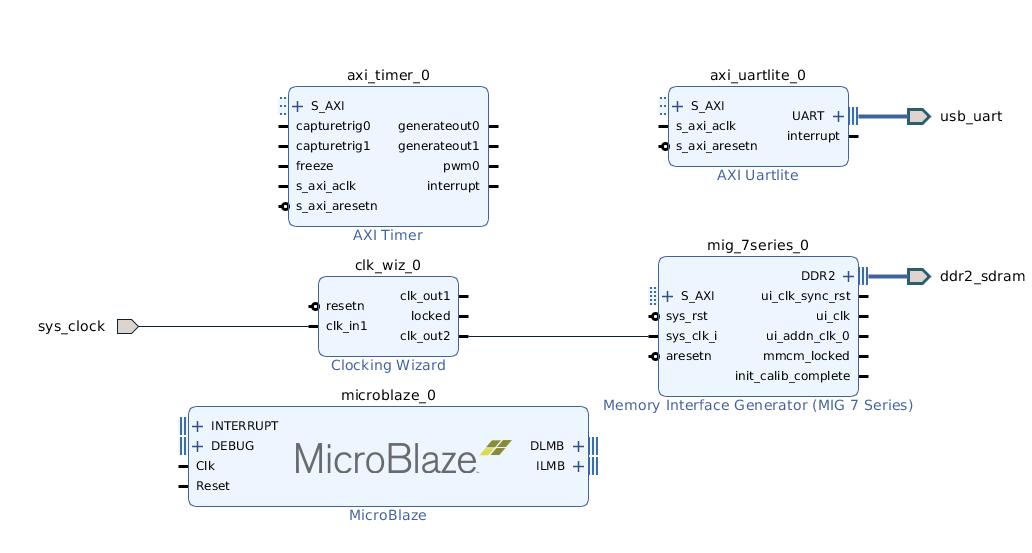
\includegraphics[width=0.8\textwidth]{Hauptteil/schritt6.png}
\caption{Neue Verbindung zwischen ClkWiz und MIG7}\label{fig:mbschritt6}
\end{figure}


Schritt 7:

Ab hier übernimmt zuerst die „Block Automation“, bei der die im nachfolgenden Bild angezeigten Einstellungen zu übernehmen sind.
Besonders wichtig ist hier die Auswahl des Interrupt Controller.

\begin{figure}[H]
\centering
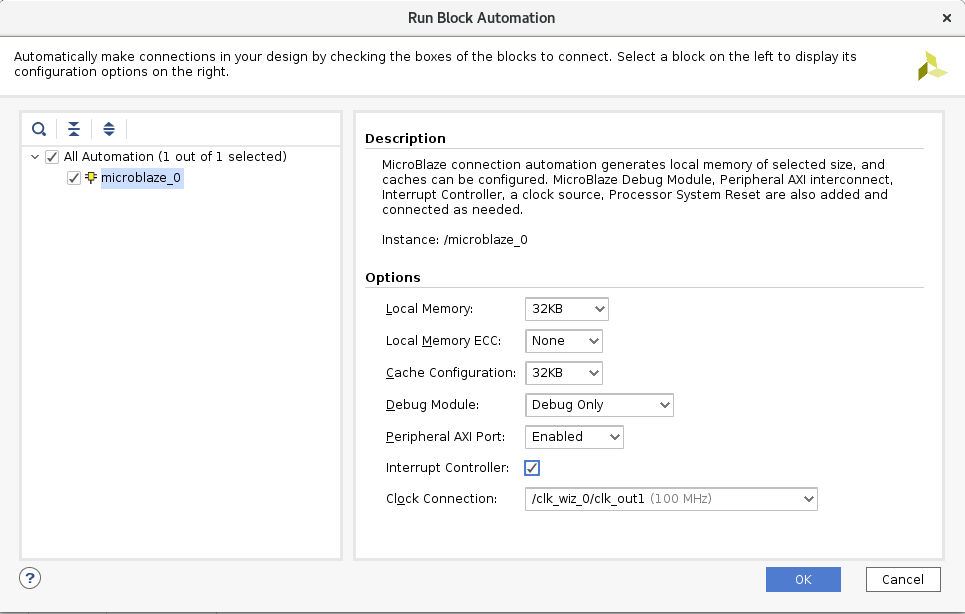
\includegraphics[width=0.8\textwidth]{Hauptteil/schritt7.png}
\caption{Einstellungen der Block Automation}\label{fig:mbschritt7}
\end{figure}


Im Anschluss wird die „Connection Automation“ gestartet und alle Bausteine ausgewählt.
Durch die Schaltfläche „Regenerate Layout“ kann das Diagram neu angeordnet werden.\\

Schritt 8:

Der angelegte Interrupt Controller ist mit einem Concat verbunden, auf dessen Eingänge manuell die Interruptleitungen des AXI Uartlite und des AXI Timers gelegt werden.
Die Verbindungen sind im folgenden Bild orange gekennzeichnet.

\begin{figure}[H]
\centering
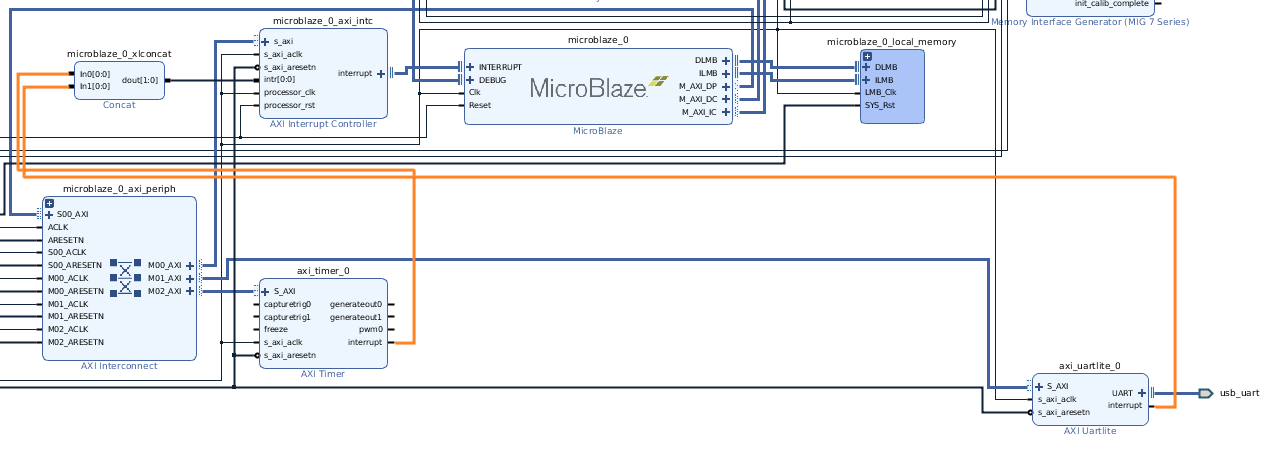
\includegraphics[width=0.8\textwidth]{Hauptteil/Schritt8.png}
\caption{Manuell erzeugte Verbindungen der Interruptleitungen}\label{fig:mbschritt8}
\end{figure}

Schritt 9:

Der Microblaze ist wie folgt durch einen Doppelklick zu konfigurieren.

\begin{figure}[H]
\centering
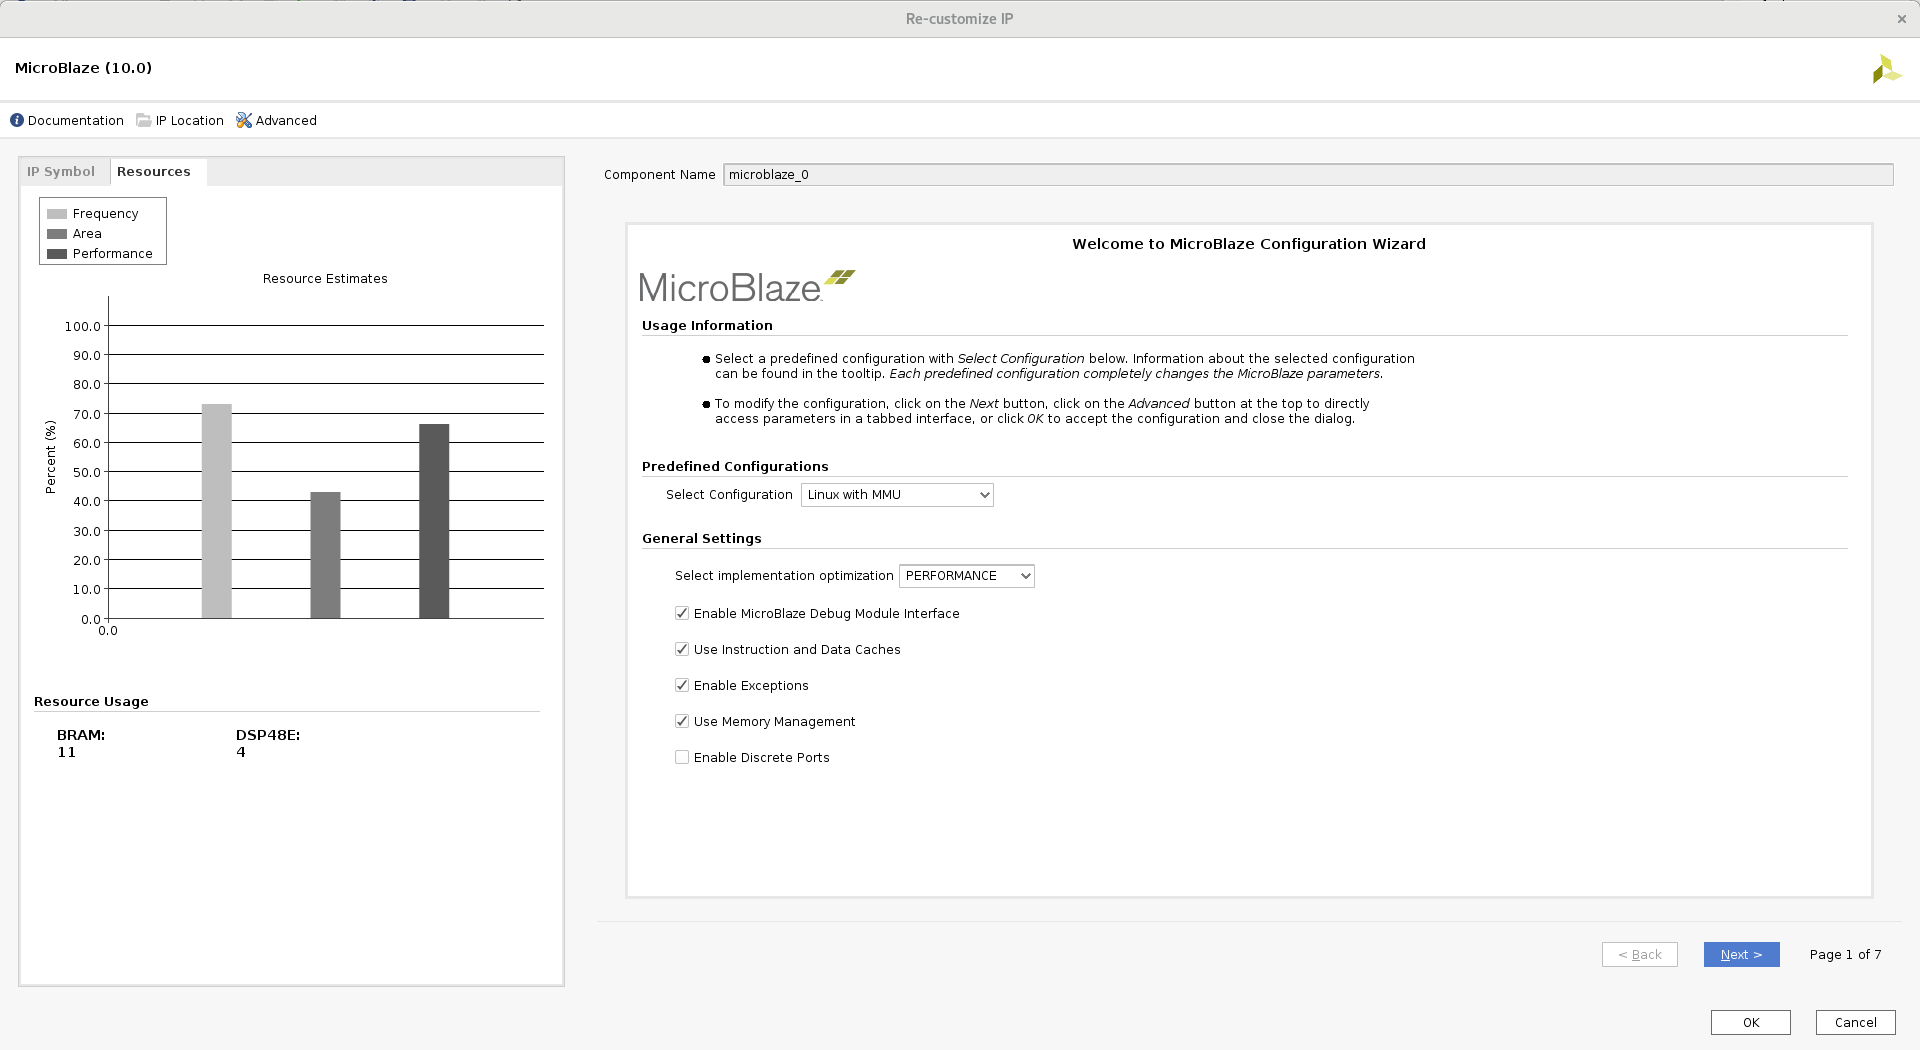
\includegraphics[width=0.8\textwidth]{Hauptteil/Schritt9.png}
\caption{Konfiguration des MicroBlaze}\label{fig:mbschritt9}
\end{figure}

Die neuen Einstellungen werden durch das Klicken des OK-Buttons übernommen.\\

Schritt 10:

Der AXI Uartlite-Baustein muss ebenfalls angepasst werden. Hierbei gilt es im Tab „IP Configuration“ die Baudrate auf 115200 anzupassen.
Diese Änderung ist mit OK zu bestätigen.

\begin{figure}[H]
\centering
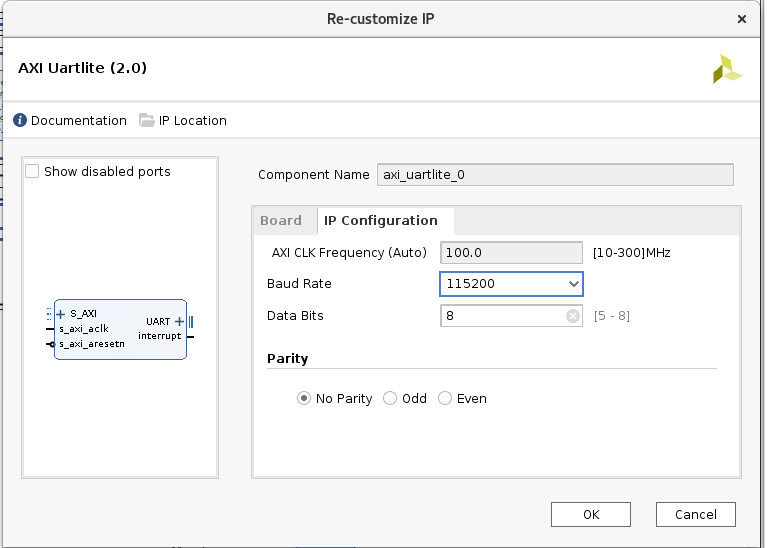
\includegraphics[width=0.8\textwidth]{Hauptteil/Schritt10.png}
\caption{Änderung der Baudrate des AXI Uartlite}\label{fig:mbschritt10}
\end{figure}

Schritt 11:

Durch klicken der rechten Maustaste auf das Design im Source-Tab wird nun der HDL Wrapper erstellt.\\

Schritt 12:

Im nächsten Schritt wird das Bitfile generiert. Dafür ist im Flow Manager der Button „Generate Bitstream“ vorgesehen.
 Die „Number of jobs“ erhöht dabei die Geschwindigkeit je nach Prozessor und verfügbaren Kernen.\\
 Im Anschluss wird über File -> Export -> Export Hardware das generierte Bitstream für die SDK, welche als nächstes gestartet wird, nutzbar gemacht.\\


Schritt 13:

Um den dazugehörigen Device Tree zu generieren, wird das Device-Tree
 Repository benötigt, welches aus dem Xilinx Github runtergeladen werden kann: https://github.com/Xilinx/device-tree-xlnx.git\\
Nach dem Entpacken wird der Ordner nun im \ac{sdk} als Repository eingebunden.
 Dies geschieht über die Schaltfläche „Xilinx Tools“ beziehungsweise Repositories.
  Hier kann nun der Pfad des Ordners nur für ein bestimmtes Projekt oder für alle Projekte hinterlegt werden.

Schritt 14:

Das Erstellen des Device-Tree geschieht über „File“ und anschließend „New“ und „Board Support Package“.
Dabei sollte nochmal die voreingestellten Parameter überprüft werden und als Board Support Package OS
devicetree ausgewählt werden.

\begin{figure}[H]
\centering
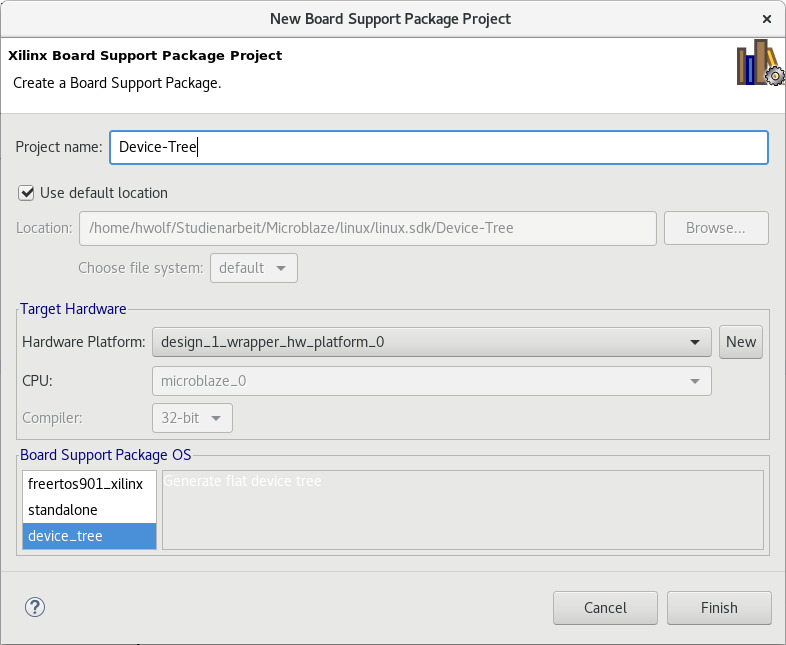
\includegraphics[width=0.8\textwidth]{Hauptteil/Schritt14.png}
\caption{Erstellen eines Device-Tree als Board Support Package}\label{fig:mbschritt14}
\end{figure}

Das folgenden Fenster kann ohne Weiteres mit OK bestätigt werden.\\


Schritt 15:

Die entstandenen \emph{.dtsi} beziehungsweise \emph{.dts}-Dateien müssen gemerged werden und in einer \emph{.dts}-Datei gespeichert werden.
Hierzu sind beide Dateien im Texteditor zu öffnen, um die \emph{.dts}
 in die \emph{.dtsi}-Datei zu kopieren.
 Die resultierende Datei wird, wie bereits erwähnt, als alleinstehende \emph{.dts}-Datei gespeichert, um später in das buildroot-Tool eingefügt zu werden.

\begin{figure}[H]
\centering
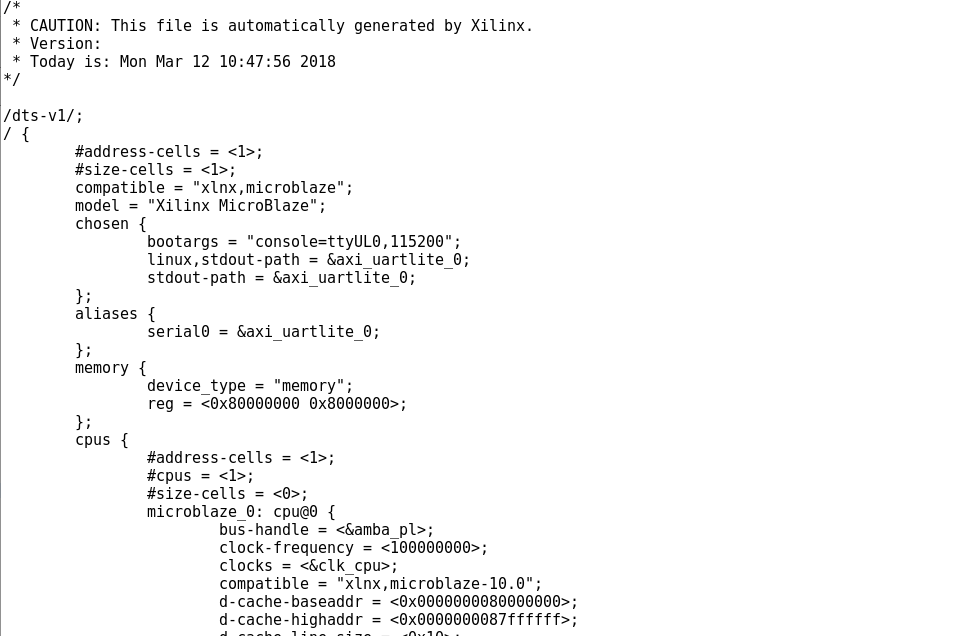
\includegraphics[width=0.8\textwidth]{Hauptteil/Schritt15.png}
\caption{Artix7.dts-Datei}\label{fig:mbschritt15}
\end{figure}

\subsection{Erstellen des Linux Image}\label{kap:microblazelinux}



Schritt 1:

Das bereits genannte Buildroot kann unter \url{https://buildroot.org/download.html} heruntergeladen werden.
Das in meiner Arbeit verwendete Buildtool besitzt die Version 2018.02.
Neben dem Buildroot werden Linux Kernel \emph{defonfig}-Dateien benötigt, welche von mir für das Nexys4 angepasst wurden und auf folgenden Github zur Verfügung stehen :

\url{https://github.com/HenW/microblaze/tree/master}

Die Dateien werden in das Verzeichnis \emph{/board/nexys/microblaze} kopiert, welche vorher neu angelegt werden müssen.
 Es ist wichtig zu beachten, dass die Basisadresse des Kernels als 0x80000000 gesetzt ist und gegebenenfalls angepasst werden muss.


\begin{figure}[H]
\centering
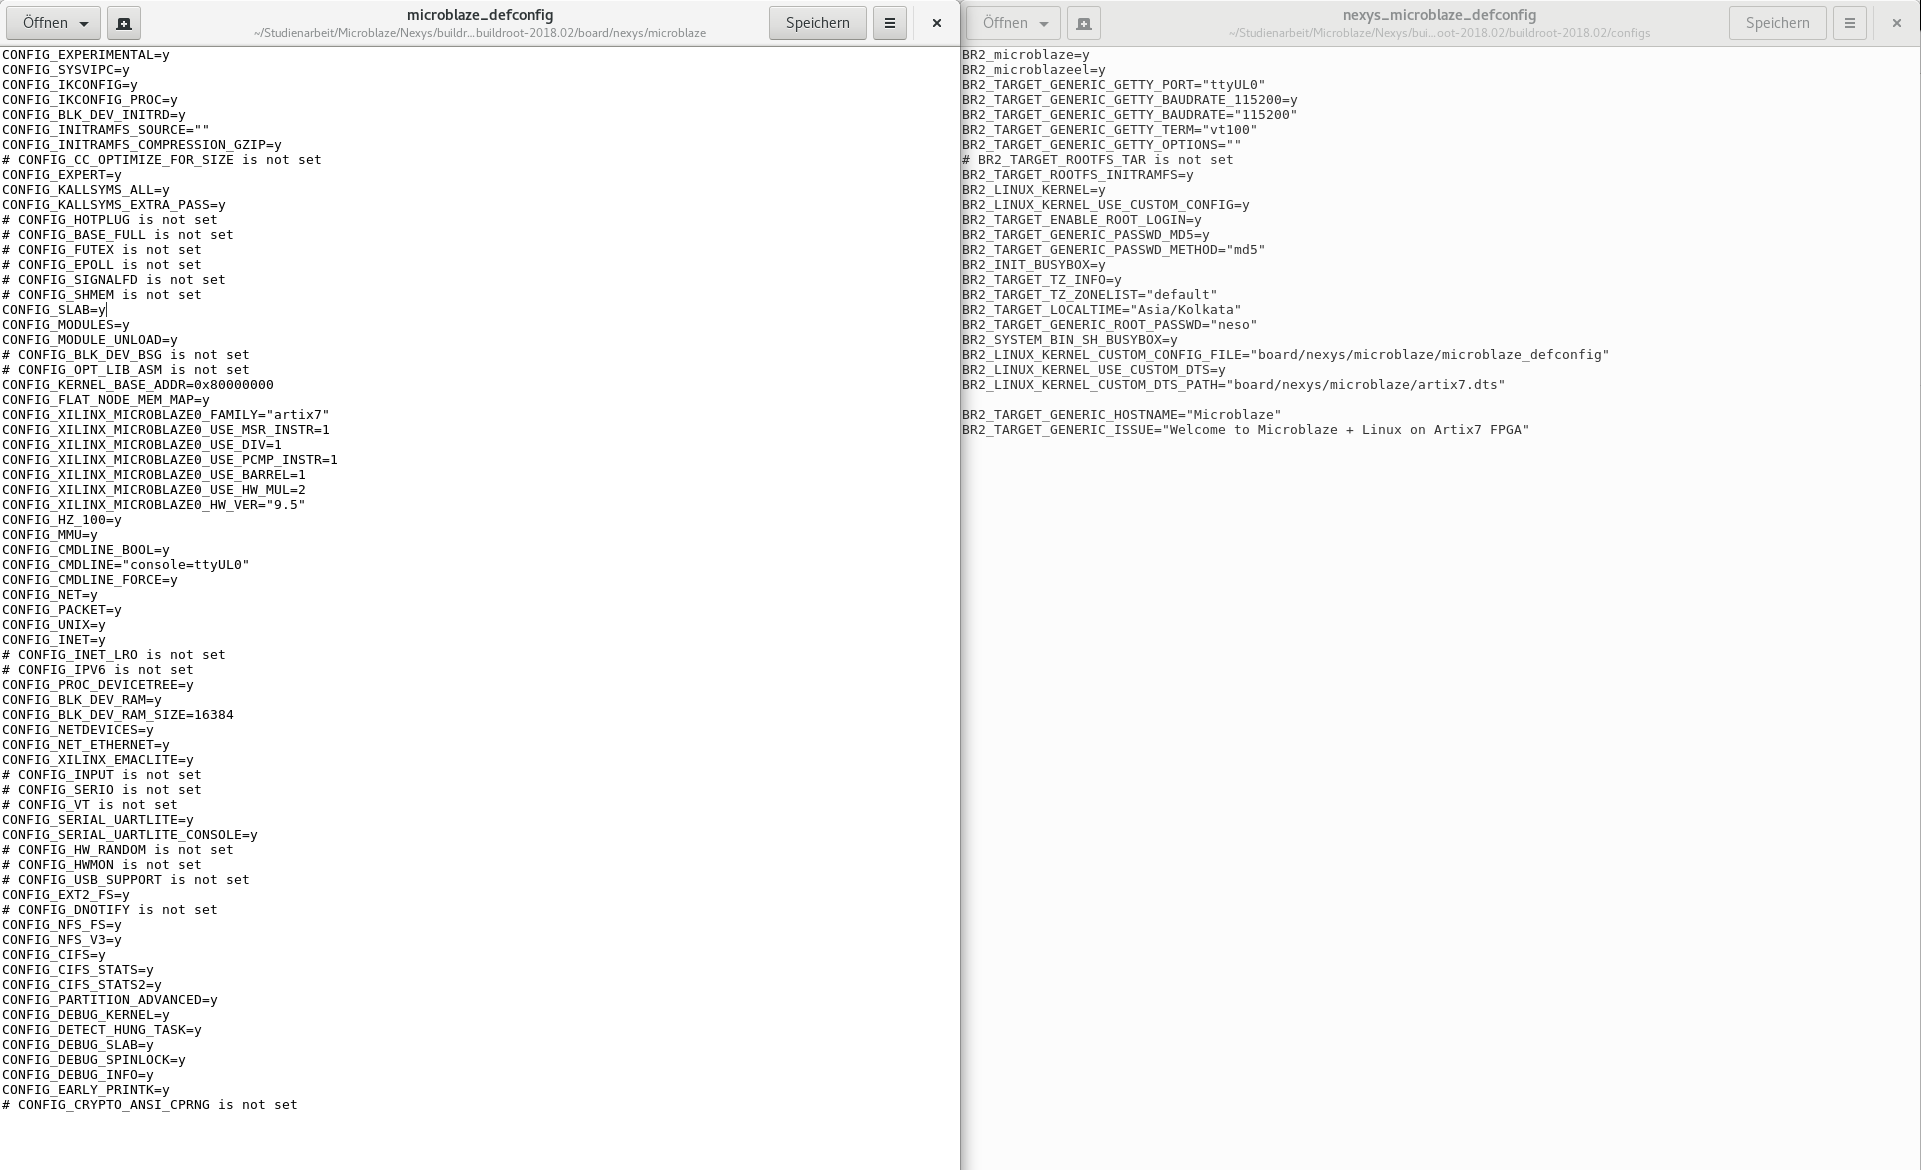
\includegraphics[width=0.8\textwidth]{Hauptteil/Schritt16.png}
\caption{Anpassung der \emph{defconf}-Dateien}\label{fig:mbschritt16}
\end{figure}

Die im vorherigen Schritt erstellte .dts-Datei muss ebenfalls in das erstellte Verzeichnis eingefügt werden.
Die Buildroot defconfig-Datei „nexys\_microblaze\_defconfig“ muss im \emph{configs}-Ordner abgelegt werden.

Schritt 2:

Nachdem das System, wie in der vorherigen Schritt beschrieben,
vorbereitet wurde, muss nun folgender Befehl mit Hilfe eines Terminals im Buildroot-Verzeichnis ausgeführt werden:

\begin{lstlisting}[caption={Generierung der \emph{defconf}-Datei},label={code:mbdefconf}]
  make nexys_microblaze_defconfig
 \end{lstlisting}


Dieser Befehl erzeugt eine sogenannte .config Datei für das zugehörige buildroot.

Schritt 3:

Um den Kernel und das passende Filesystem zu erstellen, wird der Befehl

\begin{lstlisting}[caption={Erstellung des Kernels},label={code:mbkernel}]
  make
   \end{lstlisting}

benötigt. Dieser Vorgang benötigt je nach Rechenleistung einige Minuten.
Nach erfolgreichem Abschluss des Vorgangs wird eine „simpleImage.artix7“-Datei erstellt,
welche zum booten des Linux auf dem Nexys4 DDR Artix7 \ac{fpga} Modul benötigt wird.

\subsection{Ausführen des Linux Images auf dem Artix7}\label{kap:mcausführenlinux}


Das Linux Image muss jetzt in einen Ordner kopiert werden, welcher im Anschluss über
die \ac{sdk} Shell leicht zu erreichen ist. Das \ac{FPGA}-Board wird nun mit dem Rechner über \ac{usb} verbunden und eingeschaltet.
 Über das Xilinx \ac{sdk} kann nun eine Verbindung über den korrekten Port mit der entsprechenden Baudrate (115200)
 hergestellt werden.

Schritt 1:

Um die Verbindung zu prüfen kann, nachdem das \ac{fpga}-Board programmiert wurde ein Hello World Programm ausgeführt werden. Andernfalls kann direkt im SDK über Xilinx Tools, beziehungsweise  „Launch Shell“ ein Terminal geöffnet werden.

Mit dem Befehl:

\begin{lstlisting}[caption={Öffnen des \ac{xmd}},label={code:mbxmd}]
  XMD
   \end{lstlisting}


wird eine \ac{xmd} Engine gestartet.

Anschließend wird über
\begin{lstlisting}[caption={Herstellen der Verbindung zum \acl{mb}},label={code:mbtarget}]
connect mb mdm
   \end{lstlisting}

eine Verbindung zum \ac{mb} als \ac{mdm} hergestellt.

Nun gilt es das Kernel Image auf das \ac{fpga}-Modul zu laden.
Hierzu muss innerhalb des Shells in den korrekten Ordner navigiert werden.
Über die bestehende Verbindung kann nun mit Hilfe von
\begin{lstlisting}[caption={Download des Images},label={code:mbimage}]
  dow simpleImage.artix7
   \end{lstlisting}

das Image heruntergeladen werden.



%
%
% Die oben genannten \aclp{ff} dienen zur Synchronisierung von Logikzuständen,
% sowie zur Speicherung der Zustände, zwischen zwei Taktraten.
% Am Eingang des \acl{ff} liegt entweder der Wert '\emph{1}'(True) oder
% der Wert '\emph{0}'(False) an, welcher bis zur nächsten steigenden Taktflanke
% gehalten wird (Abbildung~\ref{fig:ff}). \cite{NI}\\
%
% \begin{figure}[h]
% \centering
% \includegraphics{Hauptteil/FlipFlop.eps}
% \caption{FlipFlop-Symbol nach \cite{NI}}
% \label{fig:ff}
% \end{figure}
%
%
% In der \ac{lut} wird jeder möglichen Kombination von Eingangswerten ein festgelegter Ausgangswert
% zugewiesen (siehe Abbildung~\ref{fig:lut}).
% Durch diese Eigenschaft ist es dem \ac{clb} möglich, jede, vom Eingang abhängige, beliebige boolsche Funktion anzunehmen.
% Standardmäßig werden heutzutage 6-Input-\acp{lut} genutzt, welche, im Gegensatz zu den vorherigen 4-Input-\acp{lut},
% den Aufwand zwischen zwei \acp{lut} verringern.\cite{mikro}\\
%
% \begin{figure}[h]
% \centering
% \includegraphics{Hauptteil/LUT.eps}
% \caption{4-Input-LUT nach \cite{NI}}
% \label{fig:lut}
% \end{figure}
%
% Das \ac{fpga} verfügt als weitere Bausteine über sogenannte \acp{iob}.
% Diese werden benötigt, um Signale auf (Input), beziehungweise von dem \ac{fpga} zu senden (Output).
% Diese Blöcke sind ebenfalls konfigurierbar, sodass sie an die benötigten Standards
% angepasst werden können (CMOS/TTL).\\
%
% Dadurch, dass die Architektur mittlerweile weitestgehend standardisiert wurde,
% wird die Hardware heutzutage mithilfe einer softwareähnlichen Hardwarebeschreibungssprache beschrieben.
% Somit besitzt das System alle
% Vorteile der wiederverwendbaren und austauschbaren Bausteine bzw. Hardwarekomponenten.
% Jedoch sind \acp{fpga} in der heutigen Herstellungsart hochkomplexe Strukturen,
% die einen Mittelweg zwischen hoher Taktfrequenz, um genügend Ressourcen zu besitzen und
% preisgünstiger Herstellung meistern finden müssen. \cite{mikro}\\
%
% \section{PRHS-Framework}\label{kap:prhs}
%
% Das Kapitel \ref{kap:prhs} bezieht sich fast ausschließlich auf eine Arbeit,
% welche an der Helmut-Schmidt-Universität, Universität der Bundeswehr in Hamburg,
% genauer an der Professur für Technische Informatik in Form einer Dissertation
% entstanden ist (siehe \cite{MEckertDiss}).\\
% Das sogenannte \ac{prhs} ist zum Teil portierbar. Dabei ist es möglich, während der Laufzeit den \ac{fpga} zu
% konfigurieren, da dieser vom System simuliert wird.\cite{MEckertDiss}\\
%
% \subsubsection{PRHS-Bus}
%
%Die Verbindung zwischen der \ac{cpu}, in diesem Fall der Master und dem Speicher beziehungsweise den Peripheriegeräten,
% auch Slave genannt, wird durch den PRHS-Bus dargestellt. Das Hauptsystem, auf welches diese Arbeit aufbaut,
% besitzt spezifische Eigenschaften, welche im Nachfolgenden näher beschrieben werden.\\
%
% \begin{itemize}
%   \item Unter anderem werden dem System Datenleitungen zum Lesen(ReadData) und Schreiben(WriteData) zur Verfügung gestellt.
%   Dies bedeutet, dass die angeschlossenen Peripheriegeräte jederzeit kommunizieren können.
%   \item Eine weitere Operation ist die \emph{swap}-Operation, bei der zu erst Daten von einer bestimmten Adresse
%         gelesen werden, bevor Daten auf diese geschrieben werden. Diese Operation kann \emph{nicht} unterbrochen werden.
%   \item Es handelt sich bei dem System, mit dem gearbeitet wird, um ein 32-Bit System. Daraus folgt, dass
%         Adress- und Datenleitungen genutzt werden, die eine Bitbreite von 32 vorweisen.
%   \item Über diese Datenleitungen sollen verschieden breite Datenworte übertragbar sein. Dazu zählen \emph{word} mit
%         32-Bit, \emph{half-word} mit 16-Bit und \emph{byte} mit 8-Bit.
%   \item Essenziell wichtig war zudem, dass alle Geräte und Teilnehmer innerhalb des Bussystems über eine gleiche
%   Taktrate arbeiten.
% \end{itemize}
%
%
%
%
% Der verwendete PRHS-Bus lässt sich folgendermaßen darstellen \cite{MEckertDiss}:
%
% \begin{figure}[h]
% \centering
% \includegraphics[width=0.9\textwidth]{Hauptteil/PRHSBUS.eps}
% \caption{Aufbau des verwendeten PRHS-Busses aus \cite{ME}}
% \label{fig:PRHSBUS}
% \end{figure}
%
%
% \subsubsection{Schreib- und Leseoperationen}\label{operations}
%
% Damit die gewünschte Schreiboperation ausgeführt wird,
% muss der Master einige Parameter des PRHS-Busses setzen. Das \emph{PRHSoperation}-Signal muss
% auf  '\emph{OPWrite}' gesetzt werden, um mitzuteilen, dass
% es sich um eine Schreiboperation handelt. Des Weiteren muss vor dem Ausführen die
% \emph{PRHSaddress}-Leitung mit der gewünschten Adresse beschrieben werden. Der
% \emph{PRHSdataMaster} wird mit dem zu schreibenden Datenwort belegt. Die Breite des
% Datenwortes wird über das \emph{PRHSWidth}-Signal gesetzt. Der Master signalisiert
% über das Setzen des \emph{PRHSrequest} auf '\emph{1}' , dass die Daten auf dem Bus eine
% Anfrage darstellen.\\
% Nun überprüfen die angeschlossenen Slaves bei der nächsten steigenden Taktflanke, ob
% die in \emph{PRHSaddress} hinterlegte Adresse in ihrem Bereich liegt. Das angesprochene
% Gerät quittiert den Request, in dem es das \emph{PRHSdone}-Signal von '\emph{1}' auf '\emph{0}' setzt.
% Nun ist der Master wieder in der Lage neue Daten auf den gewünschten
% Bus zu legen und den \emph{PRHSrequest} zu resetten.\\
% Jegliche Daten auf dem \emph{PRHSdataSlave}-Signal werden vom Master ignoriert.
% Dies erlaubt, unnötigen Schaltaufwand innerhalb des Slaves zu verhindern.\cite{MEckertDiss}\\
% \newpage
% Grafisch dargestellt sieht eine Schreiboperation wie folgt aus :\\
%
% \begin{figure}[h]
% \centering
% \includegraphics[width=0.7\textwidth]{Hauptteil/PRHSwrite.eps}
% \caption{Darstellung der Signale einer Schreiboperation nach \cite{MEckertDiss}}
% \label{fig:PRHSBUS}
% \end{figure}
%
% Für die Leseoperation gibt es zwei Varianten. So kann der Slave im ersten Fall
% direkt antworten oder im zweiten Fall den Bus solange blockieren, bis er die Daten
% abrufen möchte. Die zweite Variante hat dadurch den klaren Nachteil, da in der Zeit
% der Bus für weitere Slaves blockiert ist. \\
% Um nun die Daten vom Slave über die \emph{PRHSdataSlave}-Leitung zu empfangen,
% muss der Master die Signale \emph{PRHSaddress}, \emph{PRHSWidth} und \emph{PRHSrequest} setzen.
% Entscheidend ist nun, dass der Master das \emph{PRHSoperation}-Signal auf '\emph{OPread}' setzt. \\
% Fallunterscheidung:\\
% \begin{enumerate}
% \item Der Slave legt seine Antwort unverzüglich auf die \emph{PRHSdataSlave}-Leitung
%       und quittiert per \emph{PRHSdone}-Signal, dass die vom Master gestellte
%       Anfrage bearbeitet wurde.(siehe Abbildung~\ref{fig:qr})
%
% \begin{centering}
% \includegraphics[width=0.7\textwidth]{Hauptteil/PRHSreadFast.eps}
% \captionof{figure}{Darstellung einer Leseoperation mit sofortiger Antwort nach \cite{MEckertDiss}}
% \label{fig:qr}
% \end{centering}
%
%
%
% \ \item Erwartet der Slave nun weitere Daten, oder muss Berechnungen durchführen, hält er das
%       \emph{PRHSdone}-Signal solange zurück und blockiert damit den Bus. Sollte nun ein Gerät
%        nicht antworten, kann es zum Absturz des Gesamtsystems kommen.(siehe Abbildung~\ref{fig:sr})\\
%
% \begin{figure}[h!]
% \centering
% \includegraphics[width=0.7\textwidth]{Hauptteil/PRHSreadSlow.eps}
% \caption{Darstellung einer Leseoperation mit verzögerter Antwort nach \cite{MEckertDiss}}
% \label{fig:sr}
% \end{figure}
%
% \end{enumerate}
%
% Dabei ist es wichtig zu erwähnen, dass diese Operationen für Geräte immer \emph{non-immediate} geschehen. Das heißt,
%  dass nach dem Senden des \emph{PRHSdone}-Signals eine Zeitverzögerung auftritt, um eine Befehlüberschneidung
%  zu verhindern. Der Nachteil besteht darin, dass somit die Operationen mehr Zeit in Anspruch nehmen.\\
%
% \section{Schnittstellen}\label{kap:schnittstellen}
%
% Damit das Nexys 4 DD-Board mit externen Geräte kommunizieren kann, müssen zum Beispiel serielle
% Schnittstellen wie RS-232 oder Bus-Systeme wie \ac{spi}  genutzt werden, welche sowohl
% vom Board, als auch vom Gerät unterstützt werden. \cite{schnittstelle}\\
% In den nachfolgenden Unterkapiteln werden beide Arten der Kommunikation beschreiben. \\
%
% \subsection{UART}\label{kap:uart}
%
% Um mit dem verwendeten \ac{gps}-Modul zu kommunizieren, wurde \ac{uart} als serielle Schnittstelle genutzt.
% Bei dieser Art der Kommunikation werden serielle Daten zwischen dem Board (\emph{Master})
% und dem \ac{gps}-Empfänger (\emph{Slave}) ausgetauscht. Dabei spielen die TxD und die RxD-Datenleitungen
% eine wichtige Rolle, da der Datenaustausch über diese Leitungen realisiert wird.\\
% Im Gegensatz zu der \ac{spi}-Schnittstelle (~\ref{kap:spi}), wird kein Clock-Signal
% übertragen um Daten zu validieren. Des Weiteren wird die Verbindung mit einer definierten
% Geschwindigkeit realisiert, der sogenannten \emph{Baudrate}. \cite{uartpdf} \\
% Die Baudrate bezeichnet dabei die Anzahl der Bits, welche pro Sekunde übertragen werden.
% Die bei dieser Arbeit genutzte Baudrate von 9600 wurde durch das genutzte \ac{gps}-Modul
% ebenso vorgegeben, wie die Übertragung von 8 Daten-Bits, keine Parität und einem einzigen Stop-Bit.\cite{pmodgps} \\
% \ac{uart} konvertiert die Bytes in serielle Bits, überträgt diese über eine einzelne Leitung
% und liest die zugehörigen Start- und Stop-Bits aus.\\
% Das sogenannte \emph{Character}(Zeichen) besteht aus einer konfigurierbaren Anzahl an Datenbits (in den meisten
% Fällen 7 oder 8), aus einem \emph{low-level} Start-Bit , einem optionalen Parity-Bit und einem
% oder mehreren logischen \emph{high-level} Stop-Bits.\\
% Das Start-Bit teilt dem Receiver mit, dass ein neues \emph{Character} empfangen wird.
% Die nächsten Bits, je nachdem wie viele Daten-Bits vorher konfiguriert wurden , stellen
% dann den Inhalt des \emph{Character} dar. Darauf folgt das optionale Parity-Bit,
% welches anzeigt, ob die Anzahl der mit '\emph{1}' belegten Daten-Bits gerade oder
% ungerade ist. Am Ende der Folge stehen dann entweder ein oder zwei  \emph{high-level } Stop-Bits,
% welche dem Receiver eindeutig signalisieren, dass die Übertragung vollständig ist. Dadurch,
% dass das Start-Bit \emph{high-level} (1) und das Stop-Bit \emph{low-level} (0) ist,
% ist immer eine klare Abgrenzung zwischen dem derzeitigen und dem folgenden \emph{Character} möglich.\\
%
% Die Datenübertragung lässt sich nach~\ref{fig:uart} darstellen.\\
%
% \begin{figure}[h!]
% \centering
% 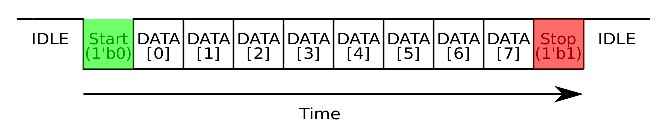
\includegraphics[width=0.8\textwidth]{Hauptteil/uart.eps}
% \caption{Datenübertragung per \ac{uart} }
% \label{fig:uart}
% \end{figure}
%
%
% \subsection{SPI}\label{kap:spi}
%
% \ac{spi} ist eines der am meisten genutzten seriellen Protokolle für \emph{inter-chip}
% oder \emph{intra-chip} Datenübertragungen. In dieser Arbeit wurde \ac{spi} dafür genutzt,
% um mit dem On-Board Beschleunigungssensor zu kommunizieren. \\
% Bei der Übertragung via \ac{spi} findet der Datenaustausch zwischen dem Master (Kernel)
% und dem Slave (Beschleunigungssensor) statt. Um einen Austausch zu gewährleisten benötigt der Master
% ein \emph{Clock}-Signal, über welches gesteuert wird, wann Daten geschrieben beziehungsweise
% gelesen werden können. So können erst Daten gesendet werden, nachdem die empfangenen
% Daten gelesen wurden. Daraus ergibt sich, dass ein Gerät im \ac{spi}-Protokoll immer ein
% Receiver und Transmitter ist und niemals nur eines von beidem.
% Für die Übertragung nutzt \ac{spi} folgende Signale:
%
% \begin{itemize}
% \item SCK (Serial Clock) Dieses Signal synchronisiert die Übertragung zwischen Master und Slave
%       und wird vom Master gesetzt.
% \item MOSI (Master Out – Slave in) Eine einfache Daten-Bit-Verbindung, welche der Master aus seinem
%       Register heraus befüllt.
% \item MISO (Master In  Slave Out) Über diese einfache Daten-Bit-Verbindung kommuniziert der
%       Slave mit dem Master, indem er die Bits aus dem Slave-Register sendet.
% \item SS (Slave Select) Wenn dies Verbindung eine '\emph{1}' überträgt und somit ein \emph{high-level}-Signal
%       wird, wird das entsprechende Gerät ausgewählt. Diese Auswahl wird durch den Master getätigt.
% \end{itemize}
%
% Die Datenübertragung basiert dabei auf einem 8-Bit Datenregister, welches sowohl der Master, als auch der
% Slave besitzt. Durch das vom Master generierte \emph{Clock}-Signal findet nun eine Übertragung statt und
% der Master schiebt sein Datenbyte auf das \emph{MOSI}-Signal. Analog dazu kann der Slave seine Daten
% wiederrum auf das \emph{MISO-Signal} legen. Wenn nun acht \emph{Clock}-Impulse generiert wurden,
% werden die Daten in das Register des Anderen geschoben. \cite{spipdf}
%
% \begin{figure}[h!]
% \centering
% \includegraphics[width=0.33\textwidth]{Hauptteil/SPI.eps}
% \caption{Datenübertragung per \ac{spi} nach \cite{spipic} }
% \label{fig:spi}
% \end{figure}
%
% \newpage
% \subsubsection{\ac{spi}-Modus}\label{kap:spimode}
%
% Über die \ac{spi}-Schnittstelle kann der Slave in verschiedenen Modi betrieben werden. Diese Modi setzen
% sich dabei aus den Werten der Parameter \ac{cpol} und \ac{cpha} nach Tabelle~\ref{tab:spimode} zusammen.
%
% \begin{table}[h]
% \centering
% \begin{tabular}{c|c|c}
% \toprule
% \textbf{Mode} & \textbf{\ac{cpol}} & \textbf{\ac{cpha}}   \\
% \midrule
% \centering
% 0 & 0 & 0 \\
% \hline
% 1 & 0 & 1 \\
% \hline
% 2 & 1 & 0 \\
% \hline
% 3 & 1 & 1 \\
% \bottomrule
% \end{tabular}
% \caption{\ac{spi}-Modi aus \cite{spimode}}
% \label{tab:spimode}
% \end{table}
%
%  In dieser Arbeit wird der \ac{spi}-Modus '\emph{0}' genutzt. Das bedeutet, dass sowohl \ac{cpol}, als auch
% \ac{cpha} den Wert '\emph{0}' annehmen. Dabei ist der Clock Idle 'Low'(\ac{cpol}='0') und die Daten werden bei der
% ersten Flanke übernommen, nach dem SS auf 'Low' gezogen wurde(\ac{cpha}='0'). Daraus ergibt sich,
% dass die ankommenden Daten bei der ersten Flanke übernommen werden, welche nur eine steigende Flanke sein kann.
% \cite{schnittstelle}
%
%
% \section{\ac{gps}}\label{kap:gps}
%
% Was in den 60er Jahren als militärisches Projekt begann, lässt sich heute in fast jedem Auto,
% Schiff, Flugzeug und Smartphone wiederfinden. Das \ac{gps}, auch \acs{navstar} genannt, wurde
% als erstes Navigationssystem auf Basis von Satellitenortung entwickelt. Nach einigen finanziellen
% und technischen Problemen läuft das System seit 1995 ohne größere Probleme.\cite{gpsabel}\\
% \ac{gps} setzt sich aus 24 Satelliten zusammen, welche auf elliptischen Bahnen um die Erde kreisen
% und sich dabei in einer Höhe von ca. 20200 km befinden. Die Satelliten sind dabei \emph{nicht} geostationär,
% sondern bewegen sich zu je vier Satelliten auf sechs unterschiedlichen Bahnen. Gegeneinander sind sie zu 60 Grad
% und gegen die Äquatorebene 55 Grad geneigt. So wird sichergestellt, dass zu jeder Zeit und an jedem Ort der
% Erde mindestens vier Satelliten nutzbar sind. \cite{gpsabel}\\
% Die Entfernungsbestimmung durch Laufzeit ist ein durchaus kompliziertes Verfahren. Die Position des Empfängers
% wird durch drei Satelliten bestimmt, indem diese Datenpakete senden, welche die aktuelle Position und die
% Sendezeit beinhalten. Da nun diese Signale mit Lichtgeschwindigkeit übertragen werden, würde es bei einem
% Fehler von einer tausendstel Sekunde zu einer Abweichung von 300 km kommen. Um die notwendige Genauigkeit zu
% gewährleisten, werden mehrere Atomuhren an Bord der Satelliten eingesetzt, die rund um die Uhr von der Erde aus
%  kontrolliert werden. Durch den Einfluss der speziellen Relativitätstheorie, dass heißt aufgrund der reduzierten Schwerkraft,
% gehen die Uhren an Bord langsamer. Dem wirkt man entgegen, indem diese Atomuhren mit einer
% niedrigeren Grundfrequenz eingestellt werden. \cite{gpsabel}\\
%
% \begin{figure}[h!]
% \centering
% \includegraphics[width=0.3\textwidth]{Hauptteil/gps.eps}
% \caption{Positionsbestimmung per GPS nach \cite{gpsabel}}
% \label{fig:gps}
% \end{figure}
%
%
%
% Die Positionsbestimmung wird anhand der kartesischen Koordinaten berechnet und angeben.
% Um das Gleichungssystem mit den Unbekannten \(X_{p}\) , \(Y_{p}\) , \(Z_{p}\) und dem Distanzfehler D zu lösen, werden
% mindestens vier Satelliten benötigt. Befindet sich nun ein Satellit bezüglich des Koordinatensystems
% auf der Position (\(X_{0}\) , \(Y_{0}\) , \(Z_{0}\)), wie in der Abbildung~\ref{fig:gps} dargestellt, wird dieser Punkt als Referenzpunkt
% für die Berechnung der anderen Satelliten genutzt. So gilt für \(R_{0}\):\\
%
% \begin{equation*}
% R_{0}=\sqrt{ (X_{p}-X_{0})^2+(Y_{p}-Y_{0})^2+(Z_{p}-Z_{0})^2}-D\\
% \end{equation*}
%
% \newpage
% \section{Pmod-\ac{gps}-Receiver}\label{kap:gpsreceiver}
%
%
% Der in dieser Arbeit genutzte GPS-Sensor ist ein \emph{PmodGPS}-Sensor der Firma Digilent Inc..\\
% Dieser kann verschiedene Systeme um die Funktion der Positionsbestimmung via Satelliten erweitern und
% besitzt des Weiteren folgende Eigenschaften:\cite{pmodgpsman}\\
% \begin{itemize}
% \item Zwei- und dreidimensionale Positionsbestimmung
% \item Hohe Empfindlichkeit (-165 dBm)
% \item Eine Genauigkeit von \(\pm\)3 Meter
% \item Aktualisierungsrate von bis zu 10 Hz
% \item Kleine Bauart (0,8 cm x 5,0 cm x 2,0 cm)
% \item \ac{nmea}-Standard für die Kommunikation
% \item Datenübertragung zum System via \ac{uart}
% \item Automatisches Wechseln zwischen interner und externer Antenne(falls vorhanden)
% \end{itemize}
%
% \begin{figure}[h!]
% \centering
% \includegraphics[width=0.45\textwidth]{Hauptteil/pmodgps.eps}
% \caption{Der Pmod \ac{gps}-Receiver nach \cite{pmodgpsman} }
% \label{fig:pmodgpsman}
% \end{figure}
%
%
% \subsection{System Block Diagram}\label{kap:gpsblock}
%
%
% Die Abbildung~\ref{fig:gpsmodblock} zeigt das System Block Diagram des \ac{gps}-Sensors.\\
%
% \begin{figure}[h!]
% \centering
% \includegraphics[width=0.6\textwidth]{Hauptteil/gpsmodblock.eps}
% \caption{System Block Diagram aus \cite{pmodgpsman} }
% \label{fig:gpsmodblock}
% \end{figure}
%
% Für die Implementierung sind jedoch nur die I/O-Signale wichtig(siehe Abbildung~\ref{tab:gpsmodtable}).
% In diesem Kapitel wird näher auf die sechs Pins des Sensors eingegangen, sowie auf den Pin, welcher zum externen
% Zurücksetzen (\emph{Reset})genutzt werden kann. Das Erweitern des Sensors mithilfe einer externen Antenne
% zur Verbesserung des Empfangs wird im nächsten Abschnitt näher erläutert.\\
%
% \begin{table}[h!]
% \centering
% \scriptsize
% \begin{tabular}{c|c|c}
% \toprule
% \multicolumn{3}{c}{\textbf{Connector J1}}\\
% \midrule
% \centering
% \textbf{Pin} & \textbf{Signal} & \textbf{Description}  \\
% \hline
% 1 & 3DF & 3D-Fix Indicator \\
% \hline
% 2 & RX & Receive  \\
% \hline
% 3 & TX & Transmit  \\
% \hline
% 4 & 1PPS & 1 Pulse Per Second \\
% \hline
% 5 & GND & Power Supply Ground \\
% \hline
% 6 & VCC & Power Supply (3.3V) \\
% \toprule
% \multicolumn{3}{c}{\textbf{Connector J2}}\\
% \midrule
% \centering
% \textbf{Pin} & \textbf{Signal} & \textbf{Description}  \\
% \hline
% 1 & \(^\sim\)RST & Reset (active low) \\
% \hline
% 2 & RTCM & DGPS data pin \\
% \bottomrule
% \end{tabular}
% \caption{Pinübersicht des \ac{gps}-Sensors nach \cite{boardman}}
% \label{tab:gpsmodtable}
% \end{table}
%
% \newpage
% Wie in der Abbildung~\ref{fig:gpsmodblock} und in der Tabelle~\ref{tab:gpsmodtable} gezeigt,
% besitzen die einzelnen Pins verschiedene Aufgaben:\cite{pmodgpsman}\\
%
%
% \begin{enumerate}
% \item \textbf{3DF}: Der sogenannte \emph{3D-Fix Indicator} gibt den Status der Positionsbestimmung
%                     des Nutzers an. Bei konstanter Positionierung ist der Wert '\emph{0}', sprich ein \emph{low-level}-Signal.
%                     Ist es nicht möglich eine Position zu bestimmen, wird das Signal jeweils abwechselnd für eine Sekunde auf
%                     '\emph{1}' beziehungsweise '\emph{0}' gesetzt.
% \item \textbf{RX/RXD}: Ermöglicht die Übertragung von seriellen Daten für Softwarekommandos oder ein
%                     mögliches Firmware Update über \ac{uart}.
% \item \textbf{TX/TXD}: Dieses Signal wird für die Übertragung von seriellen \ac{gps}-Daten via \ac{uart} genutzt,
%                     welche standardmäßig das \ac{nmea}-Format haben. Diese Informationen können anschließend in Applikationen
%                     genutzt werden.
% \item \textbf{1PPS}: Dieser Pin gibt dem Eingang des angeschlossenen System ein \emph{Puls-pro-Sekunde}-Signal, welches
%                      zur Synchronisation der \ac{gps}-Zeit dient.
% \item \textbf{GND}: Der Masse (engl. \emph{chassis ground}) ist das Potential null zugeordnet und stellt somit
%                     das Bezugspotential für alle Signal- und Betriebsspannungen dar.
% \item \textbf{VCC}: Dieser Pin dient als Gleichspannungsversorgung des Moduls, wobei der Wert zwischen 3,0 und 4,3 Volt
%                     liegen muss. Die typische Spannung beträgt 3,3 Volt.
% \end{enumerate}
%
% Das \emph{\(^\sim\)RST}-Signal, welches auf dem zweiten Pin des \emph{J2-Connector} liegt, ist ein sogenanntes
% \emph{active-low}-Signal und damit vom Sinn her invertiert. Um das Modul zu zurückzusetzen, muss demnach eine
% '\emph{0}' auf das Signal gegeben werden.\\
%
% \subsubsection{Externe Antenne}\label{kap:extern}
%
%
%
% \ Das Erweitern des Moduls um eine externe Antenne ist leicht umzusetzen. Hierfür
% wird ein \ac{sma}-Adapter benötigt, welcher dann am \emph{J4-Connector} angelötet wird.
% In dieser Arbeit wird dafür der \emph{CONSMA003.062} der Firma \emph{Linx Technologies Inc.}
% verwendet(siehe Abbildung~\ref{fig:sma}).\\
%
% \begin{figure}[h!]
% \centering
% \includegraphics[width=0.1\textwidth]{Hauptteil/sma.eps}
% \caption{Abbildung des verwendeten \ac{sma}-Adapters aus \cite{sma} }
% \label{fig:sma}
% \end{figure}
%
%
% An diesem \ac{sma}-Adapter wird nun die externe Antenne angeschraubt. Hier wird die
% \emph{ANT-GPS-SH-SMA-ND}-Antenne der Firma \emph{Linx Technologies Inc.}
% genutzt(siehe Abbildung~\ref{fig:antenne}), welche einen Frequenzbereich
% von 1570,24MHz bis 1580,42MHz abdeckt. Ddamit wird eine der \ac{gps}-Trägerfrequenzen
% abgedeckt, welche bei 1575,42MHz liegt.\cite{itwissen}\\
%
% \begin{figure}[h!]
% \centering
% \includegraphics[width=0.3\textwidth]{Hauptteil/antenne.eps}
% \caption{Abbildung der verwendeten Antenne aus \cite{antenne} }
% \label{fig:antenne}
% \end{figure}
%
% \subsubsection{Output Sentences}\label{kap:outputsentences}
%
%
% Die Daten, welche von dem \ac{gps}-Sensor auf das Datensignal gelegt werden, entsprechen dem \ac{nmea}-Standard.
% Dabei enthält ein gesamtes Datenpaket fünf verschiedene \emph{Options}. Diese \emph{Options} beinhalten verschiedene
% Informationen und sind im Anhang näher erklärt. \\
%
% \newpage
% Als Beispiel für eine der \emph{Options}, wird die \ac{gga} in Listing~\ref{code:gga} und Tabelle~\ref{tab:gga}
% erläutert.\cite{pmodgpsman}\\
%
%
% \begin{lstlisting}[caption={\emph{\ac{nmea}-Message}-Beispiel für \ac{gga} aus \cite{pmodgpsman}},label={code:gga}]
%   \$GPGGA,064951.000,2307.1256,N,12016.4438,E,1,8,0.95,39.9,M,17-8,M,,*65
% \end{lstlisting}
%
%
% \begin{table}[h]
% \centering
% \begin{tabular}{c|c}
% \toprule
% \textbf{Example} & \textbf{Description}   \\
% \midrule
% \centering
% \$GPGGA & Message ID \\
% \hline
% 064951.000 & UTC Time (hhmmss.sss) \\
% \hline
% 2307.1256 & Latitude (ddmm.mmmm) \\
% \hline
% N & N/S Indicator  \\
% \hline
% 12016.4438 & Longitude (ddmm.mmmm) \\
% \hline
% E & E/W Indicator  \\
% \hline
% 1 & Position Fix Indicator  \\
% \hline
% 8 & Satellites used \\
% \hline
% 0.95 & HDOP  \\
% \hline
% 39.9 & MSL Altitude\\
% \hline
% M & Units  \\
% \hline
% 17.8 & Geoidal Separation  \\
% \hline
% M & Units  \\
% \hline
% & Age of Diff.Corr.  \\
% \hline
% *65 & Checksum \\
% \hline
% <CR><LF> & End of message indicator  \\
% \bottomrule
% \end{tabular}
% \caption{\ac{gga}-Daten Format aus \cite{pmodgps}}
% \label{tab:gga}
% \end{table}
%
%
%
% Beim späteren Verwenden der Daten in einer Applikation(siehe Kapitel~\ref{kap:applikation}), hilft der \ac{gpsd},
% welcher die Daten aufbereitet und in \emph{structs} gespeichert zur Verfügung stellt. Dies ist der entscheidene
% Vorteil gegenüber eines direkten Datenabgriffs, ebenso wie die Möglichkeit, dass der \ac{gpsd} diese Daten
% an mehrere Applikationen verteilen kann.\\
%
% \section{\ac{gps}-Daemon}\label{kap:gpsd}
%
% Das Kapitel~\ref{kap:gpsd} beschäftigt sich mit der näheren Erläuterung und
% Implementierung des sogenannten \emph{\ac{gpsd}}. Es handelt sich hierbei um einen \emph{\ac{daemon}} ,
% welcher unter dem Betriebssystem Linux/Unix(siehe Kapitel~\ref{kap:linux}) ein Programm darstellt,
% das im Hintergrund abläuft und bestimmte Dienste, in diesem Fall \ac{gps}-Daten, zur Verfügung stellt.
% Es gibt keine direkte Interaktion mit dem Benutzer, sondern lediglich indirekte Wege, welche beispielsweise über
%  Signale oder Netzwerksockets realisiert werden. \cite{daemon}\\
%
% Der \ac{gpsd} im Speziellen stellt dem System Informationen von \ac{gps}- und \ac{dgps}-Geräten,
% sowie von \ac{ais}-Empfängern zur Verfügung.  Dabei ist er in der Lage, neben dem \ac{nmea}-Standard-Protokoll
% weitere \ac{nmea}-Dialekte, wie zum Beispiel \emph{MKT-3301}, \emph{iTrax}, \emph{Motorola OnCore},
% aber auch Binärprotokolle (\emph{Garmin},\emph{Navcom},\emph{SiRF} etc.) abzufragen und zu
% interpretieren. \cite{gpsd}\\
% Der \emph{\ac{daemon}} besitzt die Fähigkeit, Unterschiede zwischen den unterstützen \ac{gps}-Typen zu verstecken
% und kann ebenfalls Kommandos an den \ac{gps}-Sensor schicken, um gegebenenfalls die Latenz zu verringern. \cite{gpsd}\\
%
% Der spätere Aufruf des \ac{daemon} erfolgt über die Eingabe in der Kommandozeile, bei der neben dem Aufruf
% selbst noch diverse Optionen mit angehängt werden können. \cite{gpsd}\\
% Die, für diese Arbeit wichtigen Optionen, werden nun näher erklärt.\\
%
% \begin{lstlisting}[caption={Aufruf des \ac{gpsd} in der Kommandozeile},label={code:gpsd}]
%   gpsd [-b] [-n] [-N] [-D n] [-F sockfile] [-P pidfile] [-S port] [-h] device...
% \end{lstlisting}
%
% \begin{itemize}
%   \item \textbf{-b} : Stellt eine 'Nur-Lesen'-Verbindung zum \ac{gps}-Gerät her, da einige \ac{gps}-Geräte sich nicht
%                       von dem \emph{\ac{daemon}} rekonfigurieren, beziehungsweise aktualisieren lassen.
%   \item \textbf{-n} : Auf etwaige Anwendungen wird nicht gewartet, sondern die
%                       Positionsdaten ohne Nutzung oder Bestätigung versendet, sodass diese von Beginn an auf dem gewählten
%                       Port liegen.
%   \item \textbf{-N} : Wie bereits am Anfang des Kapitels angemerkt, lässt sich ein \emph{\ac{daemon}} durch Benutzereingaben
%                       im Vordergrund ausführen, um so, wenn vorhanden, Logausgaben zu bekommen.
%   \item \textbf{-F} : Es wird eine Socket-Datei erstellt, bei der die bidirektionale
%                       Softwareschnittstelle angegeben wird. Hierbei ist eine Angabe eines Speicherortes nötig.
%                       In diese Datei lassen sich dann Befehle schreiben, welche die Geräteliste des \emph{\ac{daemon}} editieren.
%   \item \textbf{-P} : Über diese Option erreicht der Nutzer, dass eine \ac{pid}-Datei erstellt wird. Hierbei wird die Angabe
%                       eines Speicherortes, sowie des Dateinamens vorausgesetzt.
%   \item \textbf{-D} : Diese Option setzt das sogenannte \emph{Debug}-Level. Es ist standardmäßig auf \emph{'0'} gesetzt
%                       und kann so zwischen \emph{'0'} und \emph{'9'} liegen. Ab \emph{Debug}-Level \emph{'2'} schreibt
%                       der \emph{\ac{daemon}} sämtliche Aktionen und eingehende Befehle in den Standard-Error, wenn er im Vordergrund
%                       läuft (siehe Option \emph{'-N'}) oder in den \emph{syslog}, wenn er im Hintergrund läuft.
%   \item \textbf{-S} : Der \emph{\ac{daemon}} bestizt die Fähigkeit, die empfangenen Daten per \ac{tcpip} im Netzwerk zur
%                       Verfügung zu stellen. Mit dieser Option lässt sich der Port explizit angeben. Wird kein Port
%                       definiert, nutzt der \emph{\ac{daemon}} standardmäßig den Port 2947.
%   \item \textbf{-h} : Wird diese Option im Aufruf genutzt, werden sämtliche Befehle und Erklärungen als Hilfe angezeigt
%   \item \textbf{-V} : Anzeige der genutzten Version. Danach wird der \emph{\ac{daemon}} beendet.
% \end{itemize}
%
% \section{Beschleunigungssensor\label{kap:accelerometer}}
%
% Bei dem ADXL362-Beschleunigungssensor handelt es sich um einen
% sogenannten \emph{On-Board},\emph{3-axis} \emph{\ac{mems}} \emph{Accelerometer}
% der Firma Analog Devices Incorporated. Er ist, wie in Abbildung~\ref{fig:boardbottom} (Nummer 2) gezeigt, auf der
% Rückseite des Nexys 4 DDR-Boards verbaut. Er bietet bei der Bewegungserkennung eine hohe Genauigkeit und misst dabei
% Beschleunigung, Neigung, Erschütterung und Vibration und stellt diese Daten etwaigen Applikationen zur
% Verfügung. Darüber hinaus besteht die Möglichkeit die Chiptemperatur auszulesen.\\
% Dabei findet er neben dem Einsatz auf dem Board weitere Anwendung in Bereichen wie \emph{Medizinischen Messgeräten},
% \emph{Spielekonsolen} oder als \emph{Alarm-} und \emph{Bewegungsmelder}.\cite{mouser}\\
% Als typische Eigenschaften weist der Sensor folgende auf :\cite{accelerometer}\\
% \begin{itemize}
%   \item Niedriger Energieverbrauch
%   \item Hohe Auflösung
%   \item Aktivitäts-/Inaktivitätsüberwachung
%   \item Versorgungsspannungsbereich: 1,8V-3,6V
%   \item Digitale SPI- und \(I^2\)C-Schnittstelle
%   \item Breiter Temperaturbereich: -40\(^\circ\)C bis +125\(^\circ\)C
% \end{itemize}
%
% Wie oben aufgeführt nutzt dieser Sensor die \ac{spi}-Schnittstelle, welche in Kapitel~\ref{kap:spi} näher
% erklärt wird.\\
%
% Der ADXL362 verfügt über zwei Betriebsarten: \emph{Measurement-Mode} für eine kontinuierliche,
%  große Bandbreitenerfassung und \emph{Wake-Up-Mode} für begrenzte Bandbreitenaktivität. Ebenfalls ist es möglich,
%  die Messung auszusetzen, indem der Sensor in den \emph{Stand-By}-Modus geschaltet wird. In dieser Arbeit findet
%  der \emph{Measurement-Mode} Anwendung, nachdem er einmal initialisiert wurde.(siehe Kapitel~\ref{kap:accelimplementierung})\\
%
% Wie bereits erwähnt, wird für die Datenübertragung eine \ac{spi}-Schnittstelle genutzt. Dabei agiert der
% Beschleunigungssensor als \emph{Slave} und somit werden die Daten des Sensors ignoriert, solange der \emph{Master}
% Daten an den Sensor schickt.\\
%  Des Weiteren wird der Sensor im \ac{spi}-Modus '\emph{0}' betrieben.(siehe ~\ref{kap:spi})\\
% Die Verbindung per \ac{spi} wird in Abbildung~\ref{fig:connectiondiagram} erläutert.\\
%
% \begin{figure}[h!]
% \centering
% \includegraphics[width=0.5\textwidth]{Hauptteil/connectiondiagram.eps}
% \caption{4-Leiter-\ac{spi}-Anschlussschema aus \cite{accelerometer} }
% \label{fig:connectiondiagram}
% \end{figure}
%
% \subsubsection{\ac{spi}-Befehle}
%
% Der \ac{spi}-Port nutzt eine \emph{Multibyte}-Struktur, wobei das erste Byte das \emph{Command} beinhaltet.
% Dafür bestizt der ADXL362 folgenden Befehlssatz:\cite{accelerometer}\\
% \begin{itemize}
%   \item \textbf{0x0A}: Register schreiben
%   \item \textbf{0x0B}: Register lesen
%   \item \textbf{0x0D}: \ac{fifo} lesen
% \end{itemize}
%
% Die \emph{Command}-Struktur lässt sich wie in Abbildung~\ref{fig:registerread} und ~\ref{fig:registerwrite} darstellen.\\
%
% \begin{figure}[h!]
% \centering
% \includegraphics[width=0.7\textwidth]{Hauptteil/registerread.eps}
% \caption{Register lesen (Befehl: 0x0B) aus \cite{accelerometer} }
% \label{fig:registerread}
% \end{figure}
%
% \begin{figure}[h!]
% \centering
% \includegraphics[width=0.7\textwidth]{Hauptteil/registerwrite.eps}
% \caption{Register schreiben (Befehl: 0x0A) aus \cite{accelerometer} }
% \label{fig:registerwrite}
% \end{figure}
%
% Ein \ac{fifo}-Read wurde in dieser Arbeit nicht praktisch umgesetzt, ist aber in \cite{accelerometer} näher erklärt.\\
%
% \subsubsection{Register Map}\label{kap:registermap}
%
% Um die gewünschten Daten über die Datensignale zu erhalten, ist das Auslesen der korrekten Register wichtig.
% Hierfür gibt es die sogenannte \emph{Register-Map}, welche sich in der kompletten Form im Anhang befindet.\\
%
% Die verwendeten Register und deren Aufgabe werden in Kapitel~\ref{kap:accelimplementierung} näher erläutert.\\
% Ergänzend zu der \emph{Register-Map} werden die Funktionen der einzelnen \emph{ADXL362}-Register in den sogenannten
% \emph{Register-Details} genauer betrachtet.
%
% \subsubsection{Achsen-Daten-Register}\label{kap:achsendatenregister}
%
% Diese Register enthalten die acht \acp{msb} der (X,Y,Z)-Achsen Beschleunigungsdaten.Angesprochen wird das Register über
% die jeweiligen Adressen(siehe~\ref{tab:achsendatenregister}).\\
%
% \begin{table}[h]
% \centering
% \begin{tabular}{c|c|c|c}
% \toprule
% \multicolumn{1}{c|}{\textbf{Achse}} & \multicolumn{1}{c|}{\textbf{Adresse}} & \multicolumn{1}{c|}{\textbf{Name}} & \multicolumn{1}{c}{\textbf{Reset}} \\
% \midrule
% \centering
% X-Achse & 0x08 & XDATA & 0x00 \\
% \hline
% Y-Achse & 0x09 & YDATA & 0x00 \\
% \hline
% Z-Achse & 0x0A & ZDATA & 0x00 \\
% \bottomrule
% \end{tabular}
% \caption{Registertabelle nach \cite{accelerometer}}
% \label{tab:achsendatenregister}
% \end{table}
%
%  So ergibt sich folgende Abbildung für die Register:\\
%
%  \begin{figure}[h!]
%  \centering
%  \includegraphics[width=0.5\textwidth]{Hauptteil/dataregister.eps}
%  \caption{Achsen Datenregister nach \cite{accelerometer} }
%  \label{fig:dataregister}
%  \end{figure}
%
%
%
% \section{Linux}\label{kap:linux}
%
%
% Das verwendete System Linux wurde als freies Betriebssystem von Linus Benedict Torvald entwickelt.
% Es basiert auf dem Unix-Modell, jedoch schrieb Torvald den sogenannten Kernel neu. Seit dem gilt
% Linux als Open-Source-Projekt und Entwickler versuchen stetig das System zu verbessern.\cite{linux}\\
% Die wohl wichtigste Eigenschaft die Linux bzw. Unix für den Einsatz beliebt machen ist die Portabilität,
% da es weitestgehend rechnerunabhängig läuft. Weitere Eigenschaften die das Betriebssystem zu einem der
%  weitverbreitetsten Systeme überhaupt gemacht haben, sind:\\\cite{linux}\\
% \begin{itemize}
% \item  \textbf{Multi-Tasking} Das parallele Nutzen verschiedener Programme erlaubt jedem Benutzer
%         gleichzeitige Aktionen durchzuführen, ohne auf den Abschluss der letzten Tätigkeit zu warten.
% \item  \textbf{Time-Sharing} Das Priorisieren von einzelnen Prozessen erlaubt es, dass mehrere
%         Prozesse gleichzeitig ablaufen, indem abwechselnd Platz im Hauptspeicher beziehungsweise in der \ac{cpu}
%         zugewiesen wird.
% \item \textbf{Sprachenvielfalt} Neben der Sprache C stellt Linux/Unix viele Programmiersprachen
%       wie C++, Java, Python und viele mehr zur Verfügung. Dadurch, dass es sich um ein Open-Source-Projekt handelt,
%       wird diese Bibliothek, je nach System, ständig erweitert.
% \item \textbf{Grafische Benutzeroberfläche} Linuxrechner, im speziellen die Anwendungen, nutzen in
%       den meisten Fällen \ac{gnome} oder \ac{kde} als grafische Oberfläche. Durch die weitverbreitete Nutzung
%       dieser Oberflächen wurden diese kontinuierlich weiterentwickelt und bieten so eine hohe Vielfalt an
%       Anpassungsmöglichkeiten.
% \item \textbf{Netzwerk} Für die Kommunikation zwischen Server und Client hat sich das Betriebssystem bewährt,
%       da es über ein umfangreiches Paket an Software verfügt. Neben den Standardprotokollen \ac{tcpip} (IPv6 wird
%       ebenfalls unterstützt), werden weitere Formate verwendet, wie zum Beispiel \ac{uucp}, welches eine simple Form
%       der Kommunikation zwischen Linux/Unix-Rechnern darstellt.
% \end{itemize}
%
% Grundsätzliche bestehen Betriebssysteme wie Linux/Unix aus drei Hauptkomponenten.
% Der \textbf{Kern} (engl. \emph{Kernel}) bildet die grundlegenden Funktionen, wie
% zum Beispiel die Organisation und Verwaltung von Speicher, der Prozesse, sowie
% Ein- und Ausgänge und sämtliche Kommunikationsaufgaben.\\
% Das \textbf{Dateisystem} (engl. \emph{File System}) ermöglicht das Speichern von Dateien
% und errichtet einen Dateibaum und ist somit für die Datenorganisation zuständig.\\
% Die dritte Komponente stellt der \textbf{Befehlsübersetzer} dar (engl. \emph{shell}),
% welcher anhand einer Befehlssprache die Kommunikation ermöglicht und dem Benutzer erlaubt
% mit sämtlichen Peripheriegeräten zu interagieren, ohne dass die im Hintergrund laufenden
% Prozesse berücksichtigt werden müssen. \cite{ubuntu}\\
%
% \newpage
% Grafisch lässt sich der Aufbau wie folgt darstellen:\\
%
% \begin{figure}[h!]
% \centering
% 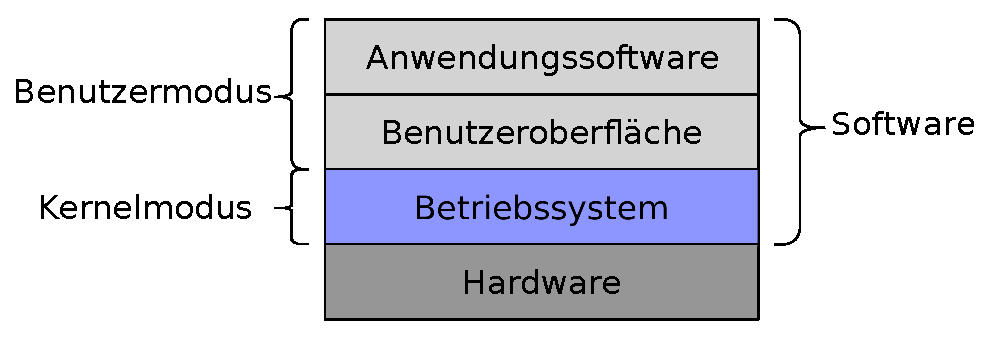
\includegraphics[width=0.8\textwidth]{Hauptteil/bs.eps}
% \caption{Aufbau der einzelnen Komponenten nach \cite{mbs}}
% \label{fig:mbs}
% \end{figure}
%
% Um nun mit den verschiedenen Geräten über eine Vielzahl von Schnittstellen kommunizieren
% zu können, benötigt jedes Gerät einen eigenen Treiber. Dieser Treiber ist im Betriebssystem
% als \emph{„Wissen“} hinterlegt und beinhaltet Information über das Gerät und dessen
% Zugriffsmöglichkeiten und wird im folgenden Unterkapitel näher erklärt. \cite{treiber}\\
% Der Anwender hat nun die Möglichkeit über die Treiber auf die Schnittstellen zuzugreifen, in dem diese vom
% Treiber gesteuert werden. Die in dieser Arbeit genutzten Schnittstellen (UART, SPI) werden in den
% Kapiteln~\ref{kap:uart} und~\ref{kap:spi} näher beschrieben.
%
% \subsection{Treiber}\label{kap:treiber}
%
% Der Treiber gilt als \emph{„Lexikon“} der jeweiligen Geräte für das Betriebssystem.
% Diese Aufgabe ist enorm wichtig für ein funktionierendes System, sodass der Stellenwert
% eines Treibers sehr hoch ist. Einfach erklärt, besteht ein Treiber aus einer Reihe von
% Funktionen, die den Zugriff auf das Gerät steuern und so eine Kommunikation ermöglichen.
% So muss für jedes Gerät ein eigener Treiber implementiert werden, der die offene
% Schnittstelle im Betriebssystemkern füllt. \\
% Dabei sind zwei Begrifflichkeiten wichtig, in die der Speicherbereich aufgeteilt wird:
% \begin{itemize}
% \item \textbf{Kernelspace} : Diese Bereich wird ausschließlich vom Kernel benutzt
% \item \textbf{Userspace} : Dieser Speicher wird von Applikationen genutzt und kann nicht,
%                           oder in Ausnahmfällen, nur eingeschränkt vom Kernel genutzt werden
% \end{itemize}
%
% Die Treiber werden grundsätzlich mit in den Kernel kompiliert oder sind als Modul dynamisch
% angelegt, um zum Kernel, während der Laufzeit, hinzugefügt zu werden. \cite{treiberbib}\\
%
% Bei der Implementierung von Gerätetreibern wird zwischen drei Gerätetypen unterschieden (\cite{treiberbib}):\\
% \begin{enumerate}
% \item \textbf{Character-Devices} Auf diese Geräte kann wie auf einen Stream von Bytes zugegriffen werden, indem
%       \ac{posix}-Funktionen genutzt werden, wie beispielsweise \emph{open()},\emph{write()},\emph{read()} oder \emph{close()}.
%       Für die Nutzung wird für jedes Gerät eine \emph{Gerätedatei} (vgl. \emph{device nodes}) angelegt.
% \item \textbf{Block Devices} Im Gegensatz zu den \emph{Character-Devices}, wird auf die \emph{Block-Devices} immer per Random Access zugegriffen.
%       Die Daten werden blockweise gelesen. Diese \emph{Block-Devices} können ein Dateisystem aufnehmen und gemountet werden.
% \item \textbf{Netzwerkschnittstellen} Netzwerkgeräte erhalten keine Gerätedatei, sondern sind in einer globalen Liste hinterlegt.
%       Der Datenaustausch findet immer asynchron statt, sodass die Netzwerkkarte jederzeit bereit sein muss Daten zu empfangen.
% \end{enumerate}
%
%
% \subsubsection{Device Tree}\label{kap:devicetree}
%
%
% Der \emph{Device-Tree} ersetzt beim \ac{arm}-Prozessor das, was beim normalen PC das \ac{bios} ist. Er beinhaltet
% Informationen, welche dem Kernel beim Booten helfen. Da das System angeschlossene Geräte nicht automatisch erkennen
% und die dazu passenden Treiber laden kann, geschieht das in dieser \emph{.dts}-Datei. Durch das Kompilieren wird daraus
% der sogennante \emph{Device} \emph{Tree} \emph{Blob}. Dieser wird zusammen mit dem Kernel vom Bootloader geladen und im
% Hauptspeicher abgelegt. Im Anschluss daran wird daraus eine Baumstruktur. In dieser sind die Geräte als Knoten angelegt
% und die dazugehörigen Treiber werden geladen. Die Verbindung zwischen Device-Tree und dem Treiber wird über eine
% eindeutige Identifikation per \emph{Compatible} festgelegt.
%
%
% \subsection{Buildroot}\label{kap:buildroot}
%
% \emph{Buildroot} ist ein Tool, welches das Erstellen eines kompletten Linux-Systems per
% \emph{Cross-Compiling} für eingebettete Systeme vereinfacht und automatisiert.  Neben dem
% \emph{cross-compiled} Toolchain können ebenfalls das \emph{Root}-Dateisystem, ein \emph{Linux-Kernel-Image}
% und ein \emph{Bootloader} für das Zielsystem erstellt werden.  In einem Konfigurationsprogramm lassen sich vor der
% Erstellung sämtliche Optionen und Erweiterungen ab- beziehungsweise anwählen. \\
% Das Tool wird größtenteils dafür genutzt, um die Systeme für andere Prozessoren, außer die klassischen x86-Prozessoren,
% zu erstellen, wie zum Beispiel \ac{arm}-Prozessoren.\\
% Der in Kapitel~\ref{kap:gpsd} näher beschriebene \ac{gpsd} lässt sich ebenfalls
% über das \emph{Buildroot}-Tool dem Gesamtsystem hinzufügen.\cite{buildroot}\\
%
%
%
% \chapter{Praktische Implementierung}\label{ch:praktischeImplementierung}
%
% Das folgende Kapitel beschreibt die eigentliche Arbeit, in welcher das \emph{NEXYS4 DDR Artix-7 FPGA}-Board
% der Firma Digilent Inc. (siehe Abbildung~\ref{fig:boardtop}) verwendet wurde.\\
% Die explizite Aufgabe dieser Arbeit ist das Anbinden des Pmod-GPS-Receivers über einen
% Pmod-Port (siehe Nummer 1 in Abbildung~\ref{fig:boardtop}) und des 3-Achsen-Beschleunigungssensors
% (siehe Nummer 2 in Abbildung~\ref{fig:boardbottom}), welcher sich auf der Rückseite des Boards befindet.\\
% Der FPGA ist in Abbildung~\ref{fig:boardtop} unter der Nummer 3 zu finden.\\
%
% \begin{figure}[h!]
% \centering
% \includegraphics[width=0.6\textwidth]{Hauptteil/boardtop.eps}
% \caption{Vorderseite des \emph{NEXYS4 DDR Artix-7 FPGA-Boards} nach \cite{digilent} }
% \label{fig:boardtop}
% \end{figure}
%
% Um nun die Konfiguration zu realisieren, wurde die Hardware mithilfe von \ac{vhdl} beschrieben.
% Bei der Synthese wird nun aus dieser Hardwarebeschreibung eine Konfigurationsdatei.\cite{mikro}\\\\
% Über den „Shared UART/JTAG USB Port“ (siehe Nummer 4 in Abbildung~\ref{fig:boardtop}) gelangt diese Konfiguration
% auf den FPGA. \\
% Das in Kapitel~\ref{kap:linux} angesprochene Betriebssystem, wird mithilfe einer Speicherkarte, über den mit
% Nummer 5 in Abbildung~\ref{fig:boardbottom} gekennzeichneten \emph{Micro-SD Connector} gebootet, welcher sich
% ebenfalls auf der Rückseite befindet.\\
% Wie bereits am Anfang des Kapitels beschrieben, wird der GPS-Sensor nun über den \emph{Pmod-Port} angeschlossen,
% welcher in Kapitel~\ref{kap:gpssensor} näher beschrieben wird, hinsichtlich Nutzung und Pinbelegung.\cite{digilent}\\
%
% \begin{figure}[h!]
% \centering
% \includegraphics[width=0.6\textwidth]{Hauptteil/boardbottom.eps}
% \caption{Rückseite des \emph{NEXYS4 DDR Artix-7 FPGA}-Boards nach \cite{digilent} }
% \label{fig:boardbottom}
% \end{figure}
%
% \section{Anbindung des \ac{gps}-Sensors}\label{kap:gpsimplementierung}
%
% Das Modul, welches eine Positionsbestimmung anhand von \ac{gps}-Daten ermöglichen soll, muss, bevor es verwendet
% werden kann zuerst angebunden werden. Dafür gibt es eine Beschreibung für die physische Anbindung der Hardware in
% Kapitel~\ref{kap:gpssensor} und eine für die logische Anbindung durch einen Treiber in Kapitel~\ref{kap:gpstreiber}.
%
%
% \subsection{Verbindung des GPS-Receivers mit dem \ac{fpga}}\label{kap:gpssensor}
%
% Auf der Seite der Hardware wird der Pmod-GPS-Receiver an einen der sogenannten \emph{Pmod-Ports}
% (siehe Nummer 1 in Abbildung~\ref{fig:boardtop}) gesteckt. Diese Ports bestehen aus insgesamt
% zwölf '\emph{Female Connectors}', wovon jeweils zwei Pin 3,3 Volt VCC Signale
% (Pin 6 und 12 nach Abbildung~\ref{fig:pmodport}) darstellen. Des Weiteren verfügt der Port über
% zwei \emph{Ground}-Signale (Pin 5 und 11 nach Abbildung~\ref{fig:pmodport}), sowie insgesamt acht
% logische Signale (siehe Abbildung~\ref{fig:pmodport}). Die bereits genannten \emph{VCC}- und \emph{Ground}-Pins
% können bis zu einem Ampere zur Verfügung stellen.\cite{boardman}\\
%
% \begin{figure}[h!]
% \centering
% \includegraphics[width=0.6\textwidth]{Hauptteil/pmodport.png}
% \caption{Übersicht der Pmod-Port-Pins und deren Funktion aus \cite{boardman} }
% \label{fig:pmodport}
% \end{figure}
%
% Um nun die korrekte Verbindung zum Board sicherzustellen, muss über das sogenannte \emph{UCF}-File
% eine Pinzuweisung getätigt werden. Die benötigte Pinzuordnung lässt sich dem Datenblatt des Boardes
% entnehmen(siehe Abbildung~\ref{tab:pmodporttable})\cite{boardman}\\
%
%
% \begin{table}[h]
% \centering
% \begin{tabular}{c|c|c|c|c}
% \toprule
% \textbf{Pmod JA} & \textbf{Pmod JB} & \textbf{Pmod JC}  & \textbf{Pmod JD} & \textbf{Pmod XDAC}\\
% \midrule
% \centering
% JA1: C17 & JB1: D14 & JC1: K1 & JD1: H4 & JXADC1: A13(AD3P) \\
% \hline
% JA2: D18 & JB2: F16 & JC2: F6 & JD2: H1 & JXADC2: A15(AD10P) \\
% \hline
% JA3: E18 & JB3: G16 & JC3: J2 & JD3: G1 & JXADC3: B16(AD2P) \\
% \hline
% JA4: G17 & JB4: H14 & JC4: G6 & JD4: G3 & JXADC4: B18(AD11P) \\
% \hline
% JA7: D17 & JB7: E16 & JC7: E7 & JD7: H2 & JXADC7: A14(AD3N) \\
% \hline
% JA8: E18 & JB8: F13 & JC8: J3 & JD8: G4 & JXADC8: A16(AD10N) \\
% \hline
% JA9: F18 & JB9: G13 & JC9: J4 & JD9: G2 & JXADC9: B17(AD2N) \\
% \hline
% JA10: G18 & JB10: H16 & JC10: E6 & JD10: F3 & JXADC10: A18(AD11N) \\
% \bottomrule
% \end{tabular}
% \caption{Nexys4 DDR Pmod Pinzuordnung aus \cite{boardman} }
% \label{tab:pmodporttable}
% \end{table}
%
% Listing~\ref{code:pinzuweisung} zeigt die Einträge des \ac{gps}-Sensors im \emph{UCF}-File. \\
%
% \lstset{language=VHDL}
% \begin{lstlisting}[caption={Pmod-Port Pinzuweisung innerhalb des \emph{UCF}-Files},label={code:pinzuweisung}]
%   # GPSSensor ; --Connector JA low
%     NET "idGPS_3DF" LOC=D17 | IOSTANDARD=LVCMOS33; # JA7
%     NET "odGPStransmit" LOC=E17 | IOSTANDARD=LVCMOS33; # JA8
%     NET "idGPSreceive" LOC=F18 | IOSTANDARD=LVCMOS33; # JA9
%     NET "idGPS_PPS" LOC=G18 | IOSTANDARD=LVCMOS33; # JA10
%   #GPSSensorRST ; --Connector JB high
%     NET "oGPSReset" LOC=D14 |  IOSTANDARD=LVCMOS33; #JB1
% \end{lstlisting}
%
% In Listing~\ref{code:pinzuweisung} ist zusehen, dass hierbei sowohl der \emph{JA}-, als auch der \emph{JB}-Connector
% genutzt wurde. Die eigentliche Verbindung der einzelnen Signale des Pmod-GPS-Receivers werden über den
% \emph{JA}-Connector realisiert. Hierfür werden jedoch nur sechs Pins benötigt, sodass lediglich die untere
% Reihe tatsächlich genutzt wurde. Den einzelnen Signalen wird ein Name, sowie der dazugehörige Pin
% zugewiesen.\\
% Die Nutzung des \emph{JB}-Connectors dient lediglich zu Realisierung eines Reset-Signales, womit der
% Pmod-GPS-Receiver sich später in der Anwendung resetten lässt. \\
%
% \subsubsection{Anbindung an den PRHS-Bus}\label{kap:prhsbus}
%
% Für das Anbinden des \ac{gps}-Moduls an den \ac{prhs}-Bus wurde ein Modul angelegt, welches wiederrum aus
% zwei Komponenten besteht. Diese Anordnung ist in Abbildung~\ref{fig:gpsprhs} zu sehen, wobei die Untermodule im
% folgenden Kapitel näher in der Funktionsweise erläutert werden.\\
%
% \begin{figure}[h!]
% \centering
% \includegraphics[width=0.8\textwidth]{Hauptteil/gpsprhs.eps}
% \caption{Aufbau des \emph{GPSUART}-Moduls und dessen Anbindung}
% \label{fig:gpsprhs}
% \end{figure}
%
% \subsubsection{UARTGPS}\label{kap:uartgps}
%
% Die Abbildung~\ref{fig:gpsprhs} im vorherigen Kapitel zeigt das sogenannte \emph{UARTGPS}-Modul. Dies wird im
% Folgenden näher erklärt. Die Einzelmodule werden dann in weiteren Unterkapiteln erläutert. \\
%
% \begin{lstlisting}[caption={Entity des \emph{UARTGPS}-Moduls},label={code:uartgpsmodul}]
%   entity GPSUART is
%           [...]
%       port
%       (
%           [...]
%         -- serial Rx/Tx signals
%           idSerialIn       : in  std_logic;          --! Rx line of RS232Interface
%           odSerialOut      : out std_logic;           --! Tx line of RS232Interface
%
%           idPPS    : in std_logic; --!PPS
%           id3DF    : in   std_logic; --!3DF
%           ocRST    : out  std_logic --! Reset Controller
%       );
%   end entity;
% \end{lstlisting}
%
% Hierbei ist zu erkennen, dass die Signale \emph{idSerialIn} und \emph{odSerialOut} lediglich in dem
%  \emph{uart4prhs}-Modul (siehe Kapitel~\ref{kap:uartrsm}) verwendet werden. Die in Listing~\ref{code:uartgpsmodul}
%  angegebenen Signale (\emph{idPPS}, \emph{id3DF}, \emph{ocRST}) werden hingegen nur im Modul für das externe
%  Zurücksetzen(Reset) genutzt.(siehe Kapitel~\ref{kap:externerreset})
%
%
% \subsubsection{UART-Register State Machine(\emph{uart4prhs})}\label{kap:uartrsm}
%
% Bei der Interaktion mit dem \ac{prhs}-Bus (siehe Kapitel~\ref{kap:prhs}) befindet sich der \ac{uart}-Baustein grundsätzlich in zwei Zuständen.
% Dieser Baustein ist im genutzten System bereits vorhanden(siehe \cite{MEckertDiss}). Entweder er wartet auf eine Anfrage vom \emph{Master} (\emph{wait4request}) oder
% er hat eine Anfrage bearbeitet (\emph{requestDone}).\\
%
% \begin{lstlisting}[caption={Zustandsbeschreibung},label={code:zustand}]
%   type uartRegFSMstates is (wait4request, requestDone)
%   signal sState : uartRegFSMstates;
%
% \end{lstlisting}
%
%  Befindet er sich im erstgenannten Zustand, überprüft er bei jeder steigenden Taktflanke des
%  Systemtaktes (\emph{iSysClk}), ob eine Anfrage seitens des Masters vorliegt (\emph{iePRHSrequest}=\emph{'1'}). Des Weiteren ist
%  anhand der Adresse zu prüfen, an wen diese Anfrage gerichtet ist.
%  \begin{lstlisting}[caption={Abgleichen der Adresse},label={code:adressabgleich}]
%    scRequest4me <= '1' when iePRHSrequest = '1' and ((icPRHSaddress and GEN_AddressMask) = GEN_BaseAddress)
%                      else '0';
%
%  \end{lstlisting}
%  Nachdem die Operation ausgeführt wurde, wechselt der Zustand(\emph{sState}) wieder auf \emph{wait4request} und
%  setzt \emph{rcDriveBus} auf '\emph{0}'.\\
%  Befindet sich nun die passende Basisadresse auf dem \emph{GEN\_BaseAddress}-Signal, erkennt das System,
%  dass die Anfrage an diese Interaktion gerichtet ist.\\
%
%  \begin{lstlisting}[caption={Basisadresse + \emph{Adressoffset}='\emph{0}' },label={code:offset0}]
%             case icPRHSaddress(3 downto 0) is
%                 when "0000" =>
%                     rdPRHSdataSlave <= X"000000" & idDataRcvd;
%                     -- OPread or OPswap --> read from RxFifo
%                     if icPRHSoperation /= OPwrite then
%                         oeReadEn        <= '1';
%                     end if;
%                     -- OPwrite or OPswap --> write to  TxFifo
%                     if icPRHSoperation /= OPread then
%                         oeWriteEn       <= '1';
%                     end if;
%  \end{lstlisting}
%
%  Nach Listing~\ref{code:offset0} werden, je nachdem welches \emph{icPRHSoperation}-Signal auf dem Bus liegt,
%  entweder Daten vom \emph{Lese-\ac{fifo}} gelesen oder Daten in den \emph{Schreibe-\ac{fifo}} geschrieben.
%
%  \begin{lstlisting}[caption={Basisadresse + \emph{Adressoffset}='\emph{4}' },label={code:offset4}]
%                  when "0100" =>
%                     rdPRHSdataSlave <= sdStatus;
%                     if icPRHSoperation /= OPread then
%                         rIntDisable     <= idPRHSdataMaster(12);
%                     end if;
%
%  \end{lstlisting}
%
% Mit dem \emph{Adressoffset}='\emph{4}' bekommt das \emph{rdPRHSdataSlave}-Signal den derzeitigen \emph{sdStatus} zugewiesen
% und sofern es sich nicht um eine \emph{OPread}-Operation handelt, wird das 12. Bit des \emph{idPRHSdataMaster}
% an das Signal '\emph{rIntDisable}' übergeben.\\
%
% \begin{lstlisting}[caption={Basisadresse + \emph{Adressoffset}='\emph{8}' },label={code:offset8}]
%                 when "1000" =>
%                     rdPRHSdataSlave <= rdBaudRate;
%                     if icPRHSoperation /= OPread then
%                         rdBaudRate <= idPRHSdataMaster;
%                     end if;
%                 when others =>
%  \end{lstlisting}
%
% \newpage
%
% Im dritten Fall (\emph{Adressoffset}='\emph{8}') wird je nach Operation entweder die Baudrate an den Slave übergeben,
% oder die neue Baudrate vom Master gesetzt. \\
%
%
% Daraus ergibt sich bei der Betrachtung von \emph{icPRHSaddress} und \emph{icPRHSoperation} folgende Tabelle~\ref{tab:ereignisse}.
%
% \begin{table}[h]
% \centering
% \begin{tabular}{c|c|c}
% \toprule
% \multicolumn{1}{c|}{\textbf{Adressoffset}} & \multicolumn{1}{c|}{\textbf{Operation}} & \multicolumn{1}{c}{\textbf{Ereignis}} \\
% \midrule
% \centering
% \multirow{2}{*}{$0x00_{h}$}
%    & /= OPwrite & Lesen von Daten aus Lese-Fifo\\
%   \cline{2-3}
%    & /= OPread &  Schreibe von Daten in die Schreib-Fifo\\
% \hline
% \multirow{2}{*}{$0x04_{h}$}
%             & /=OPread & Eintrag ins Steuerregister\\
%   \cline{2-3}
%             & & Statusabfrage des Slaves\\
% \hline
%   \multirow{2}{*}{$f0x08_{h}$}
%             & /= OPread & Baudrate wird vom Master abgefragt\\
%     \cline{2-3}
%             & & Baudrate des Slaves wird gesetzt\\
% \bottomrule
% \end{tabular}
% \caption{Ereignistabelle für \ac{uart}rsm}
% \label{tab:ereignisse}
% \end{table}
%
%
%
%
%
% \subsubsection{Externer Reset(\emph{UARTprsm})}\label{kap:externerreset}
%
%
% Des Weiteren ist es möglich über die Adresse Basisadresse + \emph{Adressoffset}='\emph{100}' die übrigen
% Signale, wie \emph{3DF}, \emph{PPS}, \emph{Reset-Controller} (siehe Kapitel~\ref{kap:gpsreceiver}), auszuwerten
% oder gegebenenfalls zu steuern. Die Funktionsweise des Automaten ist analog zu der in dem vorherigen Abschnitt beschriebenen.
% Hierbei wird jedoch immer das entsprechende Bit an die letzte Stelle von \emph{rdPRHSdataSlave} angehangen.
%
%
% \begin{lstlisting}[caption={Abfrage des \ac{pps}-Signals über \emph{Adressoffset}='\emph{100}'},label={code:offset10}]
%               when "0000" =>                 -- PPS
%                 rdPRHSdataSlave <= X"0000000" & "000" & idPPS;
% \end{lstlisting}
%
% Wie in Listing~\ref{code:offset10} beschrieben, ist es möglich das \ac{pps}-Signal über den \emph{Adressoffset}='\emph{100}'
% auf das Signal \emph{rdPRHSdataSlave} zu legen.\\
% Ebenfalls ist es möglich, das \ac{3df}-Signal auszuwerten, indem es über den \emph{Adressoffset}='\emph{104}' auf die Datenleitung
% des Slaves gelegt wird (siehe Listing~\ref{code:offset14}).\\
%
%
% \begin{lstlisting}[caption={Abfrage des \ac{3df}-Signals über \emph{Adressoffset}='\emph{104}'},label={code:offset14}]
%               when "0100" =>                 -- 3DF
%                 rdPRHSdataSlave <= X"0000000" & "000" & id3DF;
% \end{lstlisting}
%
% Die Hauptfunktion jedoch ist, über den \emph{Adressoffset}='\emph{8}' einen externen \emph{Reset} zu realisieren.
% Dabei wird das entscheidene Bit hinten angehängt und an die Datenleitung des Slaves übertragen.
% Sollte jedoch über das \emph{icPRHSoperation}-Signal die Operation \emph{OPwrite}
%  aufgerufen werden, so sendet der Master den aktuellen Wert.\\
%
%
% \begin{lstlisting}[caption={Lesen und Setzen des \emph{Reset}-Signals über \emph{Adressoffset}='\emph{108}'},label={code:offset18}]
%                 when "1000" =>                 -- Reset
%                   rdPRHSdataSlave <= X"0000000" & "000" & rcReset;
%                   if icPRHSoperation /= OPread then
%                     rcReset <= idPRHSdataMaster(0);
%                   end if;
%
% \end{lstlisting}
%
%
% Daraus ergibt sich folgende Ereignistabelle:\\
% \begin{table}[h]
% \centering
% \begin{tabular}{c|c|c}
% \toprule
% \multicolumn{1}{c|}{\textbf{Adressoffset}} & \multicolumn{1}{c|}{\textbf{Operation}} & \multicolumn{1}{c}{\textbf{Ereignis}} \\
% \midrule
% \centering
% $0x100_{h}$ & - & Legen des \ac{pps}-Signals auf die Datenleitung des Slaves\\
% \hline
% $0x104_{h}$  & - & Legen des \ac{3df}-Signals auf die Datenleitung des Slaves\\
% \hline
%   \multirow{2}{*}{$0x108_{h}$}
%             & - & Legen des \emph{Reset}-Signals auf die Datenleitung des Slaves\\
%     \cline{2-3}
%             & /=OPread & Setzen des Resetbits \\
% \bottomrule
% \end{tabular}
% \caption{Ereignistabelle für \ac{uart}prsm}
% \label{tab:EreignisseReset}
% \end{table}
%
%
% \subsection{GPS-Treiber}\label{kap:gpstreiber}
%
% Wie bereits im Kapitel ~\ref{kap:treiber} erwähnt, benötigt jedes Gerät seinen eigenen Treiber, der dem \emph{Betriebssystem}
% Informationen über das Gerät zur Verfügung stellt. Da bereits ein Baustein für \ac{uart} zur Verfügung stand,
% wurde dieser lediglich in der Adressierung aktualisiert, da für den \ac{gps}-\ac{uart} ein eigener Adressenbereich
% im \emph{Device-Tree} angelegt wurde.\\
% Der nachfolgende Code zeigt die Änderungen auf und erläutert diese.\\
% Um die \emph{OFFSET}-Adressierung anzupassen,
% wird ein \emph{UART\_GPS\_OFFSET}-Makro mit dem zugehörigen Wert definiert.\\
%
% \begin{lstlisting}[caption={Anpassung des \emph{Offset}-Bereichs im Treiber},label={code:driveroffset}]
%   #define UART_GPS_OFFSET 0x108
% \end{lstlisting}
%
% \ Wie in Kapitel ~\ref{kap:linux} erläutert, wird der \ac{gps}-Sensor resettet,
% beziehungsweise \emph{aktiv} \emph{('1')} und \emph{inaktiv} \emph{('0')} geschaltet,
% indem das \emph{\(^\sim\)RST}-Signal beim Starten  und Beenden gesetzt wird. Dieses Setzen ist im Kommentar
% nochmals angegeben.\\
%
%
% \begin{lstlisting}[caption={Anpassung des \emph{Offset}-Bereichs im Treiber},label={code:driveroffset}]
%   static int PRHSgpsuart_startup(struct uart_port *port){
%     [...]
%    status = readl(port->membase + UART_STATUS_OFFSET);
%    writel(status & ~UART_INT_DISABLE, port->membase + UART_STATUS_OFFSET);
%    writel(1, port->membase + UART_GPS_OFFSET);  --Reset
%
%    return 0;
%   }
%
%   static void PRHSgpsuart_shutdown(struct uart_port *port)
%   {
%    [...]
%    status = readl(port->membase + UART_STATUS_OFFSET);
%    writel(0, port->membase + UART_GPS_OFFSET); -- Reset
%    writel(status | UART_INT_DISABLE, port->membase + UART_STATUS_OFFSET); /* disable Interrupts */
%    [...]
%   }
%
%  \end{lstlisting}
%
%
%  \subsubsection{\ac{uart}-Eintrag im Device-Tree}\label{kap:uartdevicetree}
%
%  Um Geräte über die bereits genannten Schnittstellen (\ac{spi},\ac{uart}) betreiben und nutzen zu können,
%  müssen Treiber vorhanden sein. Das folgende Listing zeigt den Eintrag in den Device-Tree(siehe Kapitel~\ref{kap:devicetree})
%  für den \ac{uart}-Baustein.\\
%
%   \begin{lstlisting}[caption={Anlegen eines \ac{uart}-Device im \emph{Device-Tree}},label={code:uartdevicetree}]
%   -- Copyright (C) 2014 Helmut-Schmidt-University
%  [...]
% /dts-v1/;
% /include/ "prhs-base.dtsi"
%
% / {
%     model = "PRHS SoC on Nexys4 DDR";
%     compatible = "prhs,nexys4ddr";
%
%     [...]
%       uartgps: serial@f3000000 {
%           compatible = "prhs,prhs-gps-uart";
%           reg = <0xf3000000 0x1000>;
%           interrupts = <42>;
%           id = <1>;
%           interrupt-parent = <&intc>;
%           clocks = <&rootClock 0>;
%         };
%
%   \end{lstlisting}
%
% Wie in Kapitel~\ref{code:uartdevicetree} zu sehen ist, wird eine serielle Schnittstelle an der Basisadresse \emph{f3000000} erstellt.
% Zur eindeutigen Identifizierung wird das \emph{Compatible} genutzt, dieses entspricht der \emph{device\_id}, welche im
% \emph{prhs\_gpsuart}-Treiber definiert wurde.\\
% Das Speicherregister erhält eine Größe von '0x1000', beginnend mit der Startadresse. \\
% Das sogenannte \emph{interrupt}-Signal sorgt dafür, dass das Betriebssystem bei der
% Ausführung einer Anweisung immer noch reagieren kann, wenn ein wichtiges Ereignis eintritt,
% wie zum Beispiel das Eintreffen von Daten, die sonst verloren gehen würden. Bei den hier
% verwendeten \emph{interrupts}, handelt es sich um sogenannte \emph{Hardware-Interrupts}, welche genutzt werden
% um Daten von angeschlossenen Geräten zu empfangen. Dafür erhält jedes Peripheriegerät
% eine \ac{irq}, welche das Gerät identifiziert.\cite{computerlexikon}
%
%
% \section{Anbindung des Beschleunigungsensors}\label{kap:implementierungaccel}
%
% Dieses Kapitel bezieht sich auf die Anbindung des in Kapitel~\ref{kap:accelerometer} beschriebenen
%  Beschleunigungssensors. Da der Sensor bereits auf dem Board implementiert ist, war keine Anbindung auf Seiten der Hardware nötig.
% Jedoch wird in Kapitel~\ref{kap:accelimplementierung} die Anbindung des Sensors auf der Seite der Hardware
% näher erklärt. Im Kapitel~\ref{kap:acceltreiber} folgt dann die Beschreibung des zugehörigen Treibers.
%
% \subsection{Verbindung des Beschleunigungssensors mit dem FPGA}\label{kap:accelimplementierung}
%
% Wie bereits zu Beginn des Kapitels erklärt, benötigt der Beschleunigungssensor keine extra Verbindung zum Board.
% Dennoch zeigt die Abbildung~\ref{fig:pinconfigaccel} die \emph{Pin}-Konfiguration des Bauteils.
%
% \begin{figure}[h!]
% \centering
% \includegraphics[width=0.3\textwidth]{Hauptteil/pinconfigaccel.eps}
% \caption{Pin Konfiguration nach \cite{accelerometer} }
% \label{fig:pinconfigaccel}
% \end{figure}
%
% Die Tabelle~\ref{tab:pinconfigaccel} zeigt die jeweiligen Funktionen der einzelnen Pins, die in Abbildung~\ref{fig:pinconfigaccel}
% dargestellt sind.
%
% \begin{table}[h]
% \centering
% \scriptsize
% \begin{tabular}{c|c|c}
% \toprule
% \multicolumn{1}{c|}{\textbf{Pin Nr.}} &  \multicolumn{1}{c|}{\textbf{Mnemonic}} & \multicolumn{1}{c}{\textbf{Beschreibung}} \\
% \midrule
% \centering
% 1 & \(V_{DD I/O}\) & Versorgungsspannung für Input/Output\\
% \hline
% 2 & NC & \emph{No Connect}. Kein Anschluss.\\
% \hline
% 3 & Reserved & Reserviert. Ohne Anschluss oder auf \ac{gnd} gelegt werden.\\
% \hline
% 4 & SCLK & \ac{spi}-Communication Clock, entspricht dem \ac{sck} im Kapitel~\ref{kap:spi}\\
% \hline
% 5 & Reserved & Reserviert. Ohne Anschluss oder auf \ac{gnd} gelegt werden.\\
% \hline
% 6 & \ac{mosi} & Master Output - Slave Input. Serieller \ac{spi}-Dateneingang\\
% \hline
% 7 & \ac{miso} & Master Input - Slave Output. Serieller \ac{spi}-Datenausgang\\
% \hline
% 8 & \(\bar{CS}\) & Chip Select, entspricht im Kapitel~\ref{kap:spi} dem \ac{ss}\\
% \hline
% 9 & INT2 & Zweites Interrupt Signal.Ebenfalls Eingang für synchronisiertes Abtasten. \\
% \hline
% 10 & Reserved & Reserviert. Ohne Anschluss oder auf \ac{gnd} gelegt werden.\\
% \hline
% 11 & INT1 & Erstes Interrupt Signal. Ebenfalls für externes \emph{clocking}. \\
% \hline
% 12 & \ac{gnd} & Masse (engl. chassis ground)\\
% \hline
% 13 & \ac{gnd} & Masse (engl. chassis ground)\\
% \hline
% 14 & \(V_{S}\) & Versorgungsspannung\\
% \hline
% 15 & NC & \emph{No Connect}. Kein Anschluss.\\
% \hline
% 16 & \ac{gnd} & Masse (engl. chassis ground)\\
% \bottomrule
% \end{tabular}
% \caption{Pin-Funktions-Beschreibung nach \cite{accelerometer}}
% \label{tab:pinconfigaccel}
% \end{table}
%
%
% \subsubsection{UCF-File}\label{kap:ucf}
%
%
% Für die Signalidentifikation bezüglich des \ac{fpga}-Boards, muss, wie beim \ac{gps}-Sensor, ein Eintrag in dem \emph{UCF}-File erstellt werden.
% (siehe Kapitel~\ref{kap:gpssensor})\\
% \begin{lstlisting}[caption={Beschleunigungssensor Pinzuweisung innerhalb des \emph{UCF}-Files},label={code:pinzuweisungbeschleunigung}]
%   # Accelerometer
%   NET "acl_miso" LOC=E15 | IOSTANDARD=LVCMOS33; #IO_L11P_T1_SRCC_15 MISO
%   NET "acl_mosi" LOC=F14 | IOSTANDARD=LVCMOS33; #IO_L5n_T0_AD9N_15 MOSI
%   NET "acl_sclk" LOC=F15 | IOSTANDARD=LVCMOS33; #IO_L14P_T2_SRCC_15 Serial Clock
%   NET "acl_csn"  LOC=D15 | IOSTANDARD=LVCMOS33; #IO_L12P_T1_MRCC_15 ~CS: Slave Select(Active Low)
%   NET "acl_int_one" LOC=B13 | IOSTANDARD=LVCMOS33; #IO_L2P_T0_AD8P_15 Int1
%   NET "acl_int_two" LOC=C16 | IOSTANDARD=LVCMOS33; ##IO_L20P_T3_A20_15 Int2
% \end{lstlisting}
%
%  In Listing~\ref{code:pinzuweisungbeschleunigung} werden alle Input/Output-Signale im \emph{UCF}-File des Systems hinterlegt.
%  Hierbei ist zu beachten, dass die beiden Interrupt-Signale zwar definiert werden, jedoch im weiteren Verlauf nicht
%  genutzt werden.
%
%  \subsubsection{Anbindung an den PRHS-Bus}\label{kap:Anbindungbeschleunigung}
%
%  Wie bereits der \ac{uart}-Baustein, wird der \ac{spi}-Baustein ebenfalls an den \ac{prhs}-Bus angebunden.
%  Dabei besteht ein solches \ac{spi}-Modul aus einem Master und einem Slave, wie bereits
%  im Grundlagenkapitel~\ref{kap:spi} erläutert. Ebenfalls ist dort beschrieben, dass für die Implementierung
%  der bereits vorhandene \ac{spi}-Baustein genutzt wird. \\
%  Dabei werden die beiden \emph{Register-State-Machines} zusammengeführt. Im Folgenden wird anhand des \emph{\ac{spi}-Master}
%  die Funktionsweise einer Datenübertragung via \ac{spi} verdeutlicht.\\
%
%  \begin{lstlisting}[caption={Initialzustand des \ac{spi}-Master RSM},label={code:waitingspimaster}]
%    when WAITING =>   --Initial-Zustand
% 	                if (icStart= '1') then
% 	                    odMOSI <= idByteWrite(Gen_DataLength - 1);
% 	                    state <= DATAPhaseA;
% 	                    ocReadyToSend <= '0';
% 	                    rcDataPos <= Gen_DataLength - 1;
%   \end{lstlisting}
%     Dieser \emph{Initial-Zustand} ist der Ausgangzustand, welcher am Anfang initialisiert wird oder wieder erreicht
%     wird, nachdem eine Datenübertragung erfolgreich abgeschlossen wurde. Hierbei wird das Kommando vom Master an
%     den Slave übermittelt, der zu diesem Zeitpunkt kein anderes Ereignis vorliegen hat.\\
%
% \begin{lstlisting}[caption={Byteübertragung des Masters in der \ac{spi}-Master RSM},label={code:byteübertragungmaster}]
%       when DATAPhaseA =>
%   	                state <= DATAPhaseB;
%   	                if (icCPHA = '0') then
%   	                	odByteRead(rcDataPos) <= idMISO;
%   	                else
%   	                	odMOSI <= idByteWrite(rcDataPos);
%   	                end if;
%   	                SPIClk <= not SPIClk;
%      \end{lstlisting}
% Bei dem nächsten Zustand wird ein Bit vom Master an den Slave übermittelt, da es sich beim Übertragen von Daten
% per \ac{spi} um einen Austausch von Bits handelt.\\
%  Dabei wird unterschieden, ob das \ac{cpha}-Signal '\emph{0}' ist oder nicht, da je nachdem
% die Daten bei steigender oder fallender Taktflanke eingelesen werden. \\
%
% \begin{lstlisting}[caption={Datenübertragung des Slaves in der \ac{spi}-Master RSM},label={code:datenübertragungmaster}]
%   when DATAPhaseB =>
%         if (icCPHA = '0') then
%             odMOSI <= idByteWrite(rcDataPos-1);
%           else
%             odByteRead(rcDataPos) <= idMISO;
%           end if;
%           state <= DATAPhaseA;
%           [..]
%           if rcDataPos = 0 then
%             ocReadyToSend <= '1';
%             state <= WAITING;
%           else
%             rcDataPos <= rcDataPos - 1;
%           end if;
%
%  \end{lstlisting}
%
% Hierbei wechselt der Zustand ständig zwischen \emph{DATAPhaseA} und \emph{DATAPhaseB}, da solange Bits übertragen werden,
% bis der 'Zeiger'(\emph{rcDataPos}) den Wert '\emph{0}' erreicht. Somit wird signalisiert, dass alle Bits übertragen wurden
% und der Zustand wechselt wieder in den Initialzustand. \\
%
% In dem übergeordneten \emph{spi4prhs}-Modul werden, je nach Adressoffset die einzelnen Register angesprochen.
% So ergibt sich aus der Offsetunterscheidung folgende Ereignistabelle:\\
%
% \begin{table}[h!]
% \centering
% \scriptsize
% \begin{tabular}{c|c|c|c}
% \toprule
% \multicolumn{1}{c|}{\textbf{Adressoffset}} & \multicolumn{1}{c|}{\textbf{Funktion}}  & \multicolumn{1}{c|}{\textbf{Operation}} & \multicolumn{1}{c}{\textbf{Ereignis}} \\
% \midrule
% \centering
% $0x00_{h}$ & Chip Select & OPwrite & Setzen des Chip-Select-Registers\\
% \hline
% $0x04_{h}$ & Clock Divider & OPwrite & Slave bekommt den Takt vom Master\\
% \hline
%   \multirow{2}{*}{$0x08_{h}$}
%             &  Lesen & OPread & Daten vom Slave lesen\\
%     \cline{2-4}
%             & Schreiben & /=OPread & Wenn \emph{ocReadyToSend}='\emph{1}', dann schreibt der Master und \emph{requestinprogress}\\
% \hline
% \multirow{6}{*}{$0x0C_{h}$}
%           &  &  & Setzen des Master von \emph{Power on}, \emph{CPOL} \\
%           &  Control   & OPwrite  &  und \emph{CPHA} über \\
%           &    &   &  einzelne Bits des \emph{idPRHSDataMaster}\\
%   \cline{2-4}
%           &   &   & Abrufen von Informationen von \emph{CardDetect},\\
%             & Status & /=OPwrite & \emph{WriteProtect}, \emph{Power on}, \emph{CPOL}  \\
%             &   &   &  und \emph{CPHA} über Bits von \emph{rdPRHSDataSlave}  \\
% \bottomrule
% \end{tabular}
% \caption{Ereignistabelle für \ac{spi}rsm}
% \label{tab:ereignissespi}
% \end{table}
%
% \newpage
% Innerhalb des \emph{BaseReconfTop}-Moduls\cite{MEckertDiss} wird dann das Modul als \emph{Component} deklariert und es
% werden über die verschiedenen Bus-Signale die Verknüpfungen hergestellt. Hierbei beschränken sich die Änderungen
% auf die Zuweisung der Signale, welche spezifisch für den Beschleunigungssensor sind.(Siehe Listing~\ref{code:spisignal})\\
%
% \begin{lstlisting}[caption={Zuweisung der Signale des Beschleunigungssensors},label={code:spisignal}]
%   spi4prhs1 : spi4prhs
%     generic map
%     (
%         GEN_BaseAddress  => X"f4000000" --! base address for register io mem mapping
%     )
%     port map
%     (
%         [...]
%         -- SPI SPEZIFISCH
%         odMOSI => acl_mosi, --Accelerometer-Signal
%         idMISO => acl_miso, --Accelerometer-Signal
%
%         oSClk => acl_sclk,
%         iClk => iClkG,
%          ocSS => acl_csn,
%
%          oGND1 => open,
%          icnCardDetect => '0',
%          icnWriteProtect => '0',
%          oVCC1 => open,
%          oGND2 => open,
%          oVCC2 => open,
%          DAT1 => open,
%          DAT2 => open
%          [...]
%  \end{lstlisting}
%
% Hier werden die vorher im \emph{UCF}-File deklarierten Signale der \ac{spi}-Schnittstelle zugewiesen.
%
% \section{Beschleunigungssensor-Treiber}\label{kap:acceltreiber}
%
% Für den Treiber des Beschleunigungssensors wurde ein bereits vorhandener \ac{spi}-Treiber modifiziert und
% an den Sensor angepasst. Neben der Anpassung des \emph{compatible} (siehe Listing~\ref{code:accelname}), werden,
% wie auch schon beim \ac{gps}-Sensor, Makros definiert, mit deren Hilfe eine Offsetanpassung stattfindet.\\
%
% \begin{lstlisting}[caption={Anpassung des Compatible innerhalb des Treibers},label={code:accelname}]
%   static struct of_device_id prhscommonfb_of_match[] = {
%   	{ .compatible = "prhs,prhs-accelmeter", },
%   	[...]
% \end{lstlisting}
%
% Des Weiteren wird die Struktur der \emph{file\_operations} in einem struct eindeutig hinterlegt.(siehe Listing~\ref{code:fileoperations})\\
% \begin{lstlisting}[caption={\emph{file\_operations}-Struct},label={code:fileoperations}]
%   [...]
%   .open = prhs_accel_open,
%   .release = prhs_accel_release,
%   .read = prhs_accel_read,
%   .write = prhs_accel_write,
%   .compat_ioctl = prhs_accel_ioctl,
%   .unlock_ioctl = prhs_accel_ioctl,
%   [...]
%  \end{lstlisting}
%
% In der Defintion werden Makros für die Signale \emph{Chip-Select(CS)}, \emph{Clock Divider(CLKDIV)} und \emph{Befehl(COMMAND)}
% angelegt, um später diese einfacher nutzen zu können.\\
%
% \begin{lstlisting}[caption={Definition von Makros},label={code:makrosdif}]
%   #define OFFSET_CS      0x00
%   #define OFFSET_CLKDIV  0x04
%   #define OFFSET_COMMAND 0x08
%  \end{lstlisting}
%
% Zusätzlich zu den bereits vorhandenen Funktionen innerhalb des Treibers, werden nun
% zwei Funktionen (\emph{AccelDataRead},\emph{AccelDataWrite}) hinzugefügt. In diesen Funktionen werden Unterfunktionen
% aufgerufen, sodass beim Schließen der Oberfunktion die Daten gelesen, beziehungsweise geschrieben werden.\\
%
% \begin{lstlisting}[caption={Funktion zum Lesen von Daten},label={code:acceldataread}]
%   int AccelDataRead(struct prhs_accel_privdata *drvdata, char z){
% [...]
%   	writel(0, drvdata->base + OFFSET_CS);         --Set CS 0=active
%     writel(0x0b, drvdata->base + OFFSET_COMMAND); --Set Instruction (0x0b read, 0x0a write)
%   	writel(z, drvdata->base + OFFSET_COMMAND);    --Set Register Map
%   	writel(0xff, drvdata->base + OFFSET_COMMAND); --Send Data to get Data
%   	erg = readl(drvdata->base + OFFSET_COMMAND);  --Read Data
%   	writel(1, drvdata->base + OFFSET_CS);         --Set CS 1=inactive
%   [...]
%   }
%  \end{lstlisting}
%
% In Listing~\ref{code:acceldataread} ist der genaue Ablauf einer Datenabfrage dargestellt. Nachdem der Slave über
% das \emph{Chip-Select}-Signal ausgewählt wurde, wird zu erst die Instruktion übermittelt. In der 'Lesen'-Funktion
% ist es das Register mit dem Offset '\emph{0x0b}'. Je nachdem ob nun X-,Y-,Z- oder Temperaturdaten
% ausgelesen werden sollen, wird nun das entsprechende Register per die Variable '\emph{z}' übermittelt.(Register Map siehe Anhang)\\
% Nachdem der Master den Slave ausgewählt und die Übertragung eingeleitet hat, werden die Daten synchron zum Takt des Masters
% an den Datenleitungen ausgegeben. Diese Bits werden als Byte dann
% in der Variable '\emph{erg}' gespeichert und aus der Funktion zurückgegebenen. \\\\
%
% \begin{lstlisting}[caption={Funktion zum Schreiben von Daten},label={code:acceldatawrite}]
%   int AccelDataWrite(struct prhs_accel_privdata *drvdata, char z,char y){
% [...]
%   	writel(0, drvdata->base + OFFSET_CS);              --Set CS 0=active
%     writel(0x0b, drvdata->base + OFFSET_COMMAND);      --Set Instruction (0x0b read, 0x0a write)
%   	writel(z, drvdata->base + OFFSET_COMMAND);         --Set Register Map
%     writel(y, drvdata->base + OFFSET_COMMAND);         --Send Data to get Data
%   	writel(1, drvdata->base + OFFSET_CS);              --Set CS 1=inactive
%   [...]
%   }
%  \end{lstlisting}
%
% Der Unterschied zwischen Listing~\ref{code:acceldataread} und Listing~\ref{code:acceldatawrite} liegt darin, dass
% nun eine weitere Variable in die Funktion übergeben wird('\emph{y}'). Im Gegensatz zu der \emph{AccelDataRead}-Funktion,
% wird nun der Befehl in das gewählte Register ('\emph{z}') geschrieben. Dieser wurde an die Funktion übergeben. Dies wird
% genutzt um beispielsweise Register zu resetten.\cite{accelerometer}\\
%
% \subsubsection{IOCTL()-Funktion}\label{kap:ioctl}
%
% Mit der \emph{ioctl()}-Funktion ist es möglich, den Treiber unter Linux aus dem \emph{Userspace} direkt anzusprechen.
% Diese \emph{Input-Output-Control}-Funktion ermöglicht eine
% gerätespezifische Steuerung und bietet über das Schreiben und Lesen hinaus die Möglichkeit zur Steuerung des
% Gerätes.\cite{linuxunix}\\
% Das Einbinden und die generelle Syntax sind in Kapitel~\ref{kap:erprobung} näher erklärt.\\
%
% In der Funktion \emph{prhs\_accel\_ioctl} wurden verschiedene Kommandos anhand einer Switch-Case-Funktion angelegt,
% welche je nach angegebener Register-Map-Adresse die gewünschte Operation ausführt.\\
%
% \begin{lstlisting}[caption={Switch-Case-Anweisung innerhalb der Funktion \emph{prhs\_accel\_ioctl}},label={code:prhsaccelioctl}]
%   switch (ioctl_num) {
%           case ACCEL_IOCTL_QUERY_DEV_ID: --Ausgabe der Device-ID (Register-Map-Adresse: 0x00)(ioctl_num=0x35)
%   					[...]
%   				case ACCEL_IOCTL_QUERY_XDATA: --Ausgabe der X-Achsen-Daten (Register-Map-Adresse: 0x08)(ioctl_num=0x36)
%   					[...]
%   				case ACCEL_IOCTL_QUERY_YDATA: --Ausgabe der Y-Achsen-Daten (Register-Map-Adresse: 0x09)(ioctl_num=0x37)
%   					[...]
%   				case ACCEL_IOCTL_QUERY_ZDATA: --Ausgabe der Z-Achsen-Daten (Register-Map-Adresse: 0x0A)(ioctl_num=0x38)
%   					[...]
%   				case ACCEL_IOCTL_QUERY_RST_COMMAND: --Reset (ioctl_num=0x39)
%   					AccelDataWrite(drvdata,0x1F,0x52);--Soft-Reset (Register-Map-Adresse: 0x1F)
%   					AccelDataWrite(drvdata,0x1F,0x00);--Soft-Reset (Register-Map-Adresse: 0x1F)
%   					AccelDataWrite(drvdata,0x2D,0x02);--Power_CTL in Measure-Mode (Register-Map-Adresse: 0x2D)
%   					AccelDataWrite(drvdata,0x2C,0x14);--FILTER_CTL  (Register-Map-Adresse: 0x1F)
%   					break;
%   				case ACCEL_IOCTL_QUERY_TEMP: --Ausgabe der Temperatur-Daten (Register-Map-Adresse: 0x14 und 0x15)(ioctl_num=0x40)
%   					[...]
%  \end{lstlisting}
%
% Wie in Listing~\ref{code:prhsaccelioctl} zu sehen, wird innerhalb der Applikation (siehe Kapitel~\ref{kap:applikation})
% über den Parameter \emph{ioctl\_num} die gewünschte Unterfunktion aufgerufen. So lässt sich über \emph{ioctl\_num}='0x39'
% der Sensor resetten und in den \emph{Measure-Mode} schalten. Dies muss vor der ersten Nutzung geschehen. Danach können
% sowohl die \emph{Device-ID}, als auch die Daten der Achsen und die Temperatur abgefragt werden.
%
% \subsubsection{\ac{spi}-Eintrag im Device-Tree}\label{kap:spidevicetree}
%
% Für die Kommunikation mit dem Board, muss, wie beim \ac{gps}-Sensor, ein Eintrag in den \emph{Device-Tree} erstellt werden.
%  Dieser Eintrag ist in Listing~\ref{code:spidevicetree} angegeben, wobei die Bedeutung der einzelnen Parameter
%  bereits in Kapitel~\ref{kap:uartdevicetree} näher beschrieben wurden.\\
%
% \begin{lstlisting}[caption={Device-Tree Eintrag des \ac{spi}-Bausteins},label={code:spidevicetree}]
% accelmeter: accel@f4000000{
% #address-cells = <1>;
% #size-cells = <0>;
% compatible = "prhs,prhs-accelmeter";
% reg = <0xf4000000 0x1000>;
%  \end{lstlisting}
%
%
%
% \chapter{Erprobung}\label{kap:erprobung}
% Für die Erprobung wird auf dem Board das \ac{l4prhs} als Betriebssystem gebootet, welches zuvor über den SD-Kartenslot
% auf das Board gebracht wurde. Für die abschließende Erprobung
% und Demonstration wurde eine Applikation in der Programmiersprache C entwickelt.\\
%
% \section{\ac{gps}-Sensor Erprobung}\label{kap:gpserprobung}
%
% Für die Erprobung des \ac{gps}-Sensors und zur Auswertung der Daten ist es erforderlich, zuerst den
%  \ac{gpsd} zu starten.(siehe Kapitel~\ref{kap:gpsd}) Dies geschieht über den folgenden Aufruf:\\
%
% \begin{lstlisting}[caption={Tatsächlicher Aufruf des \ac{gpsd} in der Kommandozeile},label={code:gpsduse}]
%   gpsd -b -n  -D 2 /dev/ttyGPSPRHS1
% \end{lstlisting}
%
% Der genutzte \emph{Device}-Port ist der \emph{/dev/ttyGPRSPRHS1}, welcher im System vorher angelegt und
% definiert wurde. Dieser ist bereits im genutzten System, wie in der Einführung zum
% \emph{PRHS-Framework}(siehe Kapitel~\ref{kap:prhs}) erwähnt, vorhanden und wurde nur geringfügig verändert.\cite{MEckertDiss}\\
%
% Da das \ac{gpsd}-Paket nicht nur aus dem \ac{daemon} an sich besteht, sondern auch aus diversen Applikationen, wie
% zum Beispiel dem \emph{gpsmon} und dem \emph{gpspipe}, ist es möglich die empfangenen Daten unmittelbar angezeigt
% zu bekommen, um diese Auswerten zu können.\cite{gpsd}\\
%
% \begin{lstlisting}[caption={Aufruf des \emph{gpspipe} in der Kommandozeile},label={code:gpspipe}]
%   gpspipe -r /dev/ttyGPSPRHS1
% \end{lstlisting}
%
% '\emph{gpspipe}' bietet, wie der \ac{gpsd}, eine Vielzahl an zusätzlichen Optionen beim Aufruf.\cite{gpsd}\\
% Um schnell Daten zu empfangen, beschränkt sich hier die Optionswahl auf '\emph{-r}'(\ac{nmea} Datensätze werden ausgegeben) und
% den zugehörigen Port(/dev/ttyGPSPRHS1).
% Um die Syntax hinter dem Programm zu verstehen, wurde die Demo-Applikation des Herstellers analysiert.
% Anhand dieser Analyse war es möglich den Datenabgriff und die richtige
% Darstellung in der eigenen Applikation zu implementieren (siehe Kapitel~\ref{kap:applikation}).
%
% \section{Beschleunigungs-Sensor Erprobung}\label{kap:accelerprobung}
%
% Die bereits im Kapitel~\ref{kap:acceltreiber} angesprochene \emph{ioctl()}-Funktion wird nun für den Abruf der Daten genutzt.
% Diese wird in ein, auf das nötigste reduzierte C-Programm implementiert.\\
%
% Für diese Implementierung ist das Einbinden der \emph{ioctl}-Headerdatei nötig.\\
%
% \lstset{language=C}
% \begin{lstlisting}[caption={Einbinden der \emph{ioctl()}-Headerdatei },label={code:ioctlheader}]
% #include <sys/ioctl.h>
%  \end{lstlisting}
%
% Des Weiteren lässt sich die Syntax der \emph{ioctl()}-Funktion wie folgt darstellen:\\
%
%  \lstset{language=C}
%  \begin{lstlisting}[caption={Einbinden der \emph{ioctl()}-Headerdatei },label={code:ioctlheader}]
%  int ioctl(int fd,int request,...);
%   \end{lstlisting}
%
% Dabei bezeichnet '\emph{fd}' den Parameter für den geöffneten Filedeskriptor mit dem eine Gerätedatei
% geöffnet wurde. Dieser ist eindeutig über den \emph{Dateinamen} identifizierbar.\\
%  Der zweite Parameter stellt den entsprechenden Befehl dar, welcher vom Gerät abhängt.
% In der Erprobung ist dieser als \emph{magic} bezeichnet. Der genutze Befehl '\emph{0x40}' ist im Treiber des
% Beschleunigungssensors als Makro hinterlegt (siehe Kapitel~\ref{kap:acceltreiber}) und soll für die Ausgabe des
% \emph{X-Achsen}-Wertes sorgen.\\
% Der dritte und letzte Parameter, welcher übergeben wird, ist \emph{param}. Hierbei wird die Adresse einer Variablen,
% in diesem Fall \emph{xData} übergeben. Diese Variable enthält nach dem Schließen der Funktion nun die gewünschten
% Daten.\\
%
% \lstset{language=C}
% \begin{lstlisting}[caption={Empfangen von Daten mithilfe der \emph{ioctl()}-Funktion },label={code:ioctluse}]
% [...]
%       int magic = strtol(argv[2], NULL, 16);
%       int param = strtol(argv[3], NULL, 16);
%       if ((fd = open(argv[1], O_RDWR)) < 0) {
%   	perror("open");
%   	return -1;
%       }
%       ret = ioctl(fd, magic, &param);
%       printf("ioctl return %d for magic=%x, param=%x\n", ret, magic, param);
%       while(1){
%         int xdata;
%         ioctl(fd, 0x40, &xdata);
%         printf("\r xdata = %03d", xdata);
%       }
% [...]
%  \end{lstlisting}
%
% In Listing~\ref{code:ioctluse} ist der zuvorbeschriebene Funktionsaufruf dargestellt. Dabei wird in einer dauerhaften
% \emph{while}-Schleife immer wieder die \emph{ioctl()}-Funktion aufgerufen, um die X-Achsen-Beschleunigung
% kontinuierlich dazustellen.
%
%
% \section{Demo-Applikation}\label{kap:applikation}
%
% Für die letztendliche Applikation, welche im Terminal aufgerufen wird und sowohl die Darstellung der \ac{gps}-Daten,
% als auch die des Beschleunigungssensors grafisch realisiert, werden nun beide Teile zusammengefügt.
%
% \subsubsection{ncurses}\label{kap:ncurses}
%
% Für die \ac{tui}-Umgebung wurde die freie C-Programmbibliothek \emph{ncurses}(new curses) genutzt, welche eine Darstellung
% unabhängig vom darstellenden Textterminal garantiert. So ergeben sich im fertigen Programm zwei Fenster, in denen
% die Daten dargestellt werden.(siehe Listing~\ref{code:ncurses})
%
% \lstset{language=C}
% \begin{lstlisting}[caption={Darstellung der \ac{tui} via ncurses},label={code:ncurses}]
%   //Building Monitor
%       initscr();
%       //Accelerometer
%       mvaddstr(0, 0, "+----Accelerometer-----+");
%       mvaddstr(1, 0, "|X-Data:               |");
%       mvaddstr(2, 0, "|Y-Data:               |");
%       mvaddstr(3, 0, "|Z-Data:               |");
%       mvaddstr(4, 0, "|Temp:                 |");
%       mvaddstr(5, 0, "|Temp.F:               |");
%       mvaddstr(6, 0, "+----------------------+");
%     //GPSMonitor
%       mvaddstr(0, 27, "+---------------GPS----------------+");
%       mvaddstr(1, 27, "|Latitude:                         |");
%       mvaddstr(2, 27, "|Longitude:                        |");
%       mvaddstr(3, 27, "|Altitude:                         |");
%       mvaddstr(4, 27, "|Speed:                            |");
%       mvaddstr(5, 27, "|Time:                             |");
%       mvaddstr(6, 27, "+----------------------------------+");
%       mvaddstr(8, 27, "+----------------------------------+");
%       mvaddstr(9, 27, "|Status:                           |");
%       mvaddstr(10, 27,"|Mode:                             |");
%       mvaddstr(11, 27,"+----------------------------------+");
%  \end{lstlisting}
%
% \subsubsection{Darstellung der \ac{gps}-Daten}\label{kap:darstellunggps}
%
%
% Um nun die Daten des \ac{gps}-Sensors zu empfangen und in die \emph{ncurses}-Umgebung einzupflegen, müssen diese
% Daten zuallererst in ein passendes struct(\emph{gps\_data}) gepackt werden. \\
%
% \lstset{language=C}
% \begin{lstlisting}[caption={Erstellen eines Structs für die \ac{gps}-Daten},label={code:gpsstruct}]
% struct gps_data_t gps_data;
%  \end{lstlisting}
%
% Als nächstes wird mithilfe einer \emph{if}-Abfrage sichergestellt, dass der \ac{gpsd} aktiv ist
% und Daten an den Port \emph{localhost} sendet. Ist dies nicht der Fall, wird das Programm mit
% einer Fehlerausgabe beendet.(Listing~\ref{code:portopen})\\
%
% \lstset{language=C}
% \begin{lstlisting}[caption={Überprüfung ob der \ac{gpsd} aktiv ist},label={code:portopen}]
%   if ((rc = gps_open("localhost", "2947", &gps_data)) == -1) {
%       printf("code: %d, reason: %s\n", rc, gps_errstr(rc));
%       return EXIT_FAILURE;
%   }
%  \end{lstlisting}
%
% Nun wird die \ac{gpsd}-interne Funktion \emph{gps\_stream} aufgerufen und die Adresse des structs übergeben, welches
% am Anfang des Programms initialisiert wurde.\\
%
% \lstset{language=C}
% \begin{lstlisting}[caption={Aufruf der \emph{gps\_stream}-Funktion und Übergabe der Adresse des structs },label={code:gpsstream}]
% gps_stream(&gps_data, WATCH_ENABLE | WATCH_JSON, NULL);
%  \end{lstlisting}
%
% Alles Weitere nach dem Aufruf der Funktion wird nun innerhalb einer Endlosschleife(\emph{while(1)}) implementiert.
% Nachdem die Daten des Beschleunigungssensor abgerufen wurden, folgt nun die Abfrage der \ac{gps}-Daten.\\
%
% \lstset{language=C}
% \begin{lstlisting}[caption={Abruf der \ac{gps}-Daten innerhalb einer Endlosschleife},label={code:gpsdata}]
%   if (gps_waiting (&gps_data, 2000000)) { //wait for 2 seconds to receive data
%       if ((rc = gps_read(&gps_data)) == -1) {   //read data
%           printf("error occured reading gps data. code: %d, reason: %s\n", rc, gps_errstr(rc));
%       } else {
%       [...]
%  \end{lstlisting}
%
% Nun werden die im struct gespeicherten Daten in die \emph{ncurses}-Umgebung eingebettet.\\
%
% \lstset{language=C}
% \begin{lstlisting}[caption={Implementierung der \ac{gps}-Daten in die \emph{ncurses}-Umgebung},label={code:dispgpsdata}]
%   // Display data from the GPS receiver.
%      if ((gps_data.status == STATUS_FIX) &&
%          (gps_data.fix.mode == MODE_2D || gps_data.fix.mode == MODE_3D) &&
%          !isnan(gps_data.fix.latitude) &&
%          !isnan(gps_data.fix.longitude)) {
%              [...]
%              mvprintw(1,39, "%f",gps_data.fix.latitude);
%              mvprintw(2,39,"%f",gps_data.fix.longitude);
%              mvprintw(3,39,"%f",gps_data.fix.altitude);
%              mvprintw(4,39,"%f",gps_data.fix.speed);
%              mvprintw(5,34,"%s", asctime(gmtime(&test)));
%              mvprintw(9,36,"Receiving Data!");
%              switch(gps_data.fix.mode){
%                case MODE_2D:
%                  mvprintw(10,36 , "2D");
%                  break;
%                case MODE_3D:
%                  mvprintw(10,36 , "3D");
%                  break;
%                default:
%                  mvprintw(10,36 , "NO FIX");
%                  break;
%                }
%
%      } else {
%          mvprintw(9,36,"No GPS Data!");
% [...]
%   refresh();
%   usleep(1000);
%  \end{lstlisting}
%
% \subsubsection{Darstellung der Daten des Beschleunigungssensors}\label{kap:darstellungaccel}
%
% Die Daten des Beschleunigungssensors werden innerhalb der Endlosschleife kontinuierlich abgerufen, indem für
% die jeweilige Achse, beziehungsweise für die Temperatur die entsprechenden Parameter an die \emph{ioctl()}-Funktion
% übergeben werden. \\
% Bevor jedoch das Programm die \emph{while}-Schleife erreicht, muss der Sensor in den \emph{Measurement-Mode} geschaltet
% werden.(siehe dazu Kapitel~\ref{kap:acceltreiber})\\
%
% \lstset{language=C}
% \begin{lstlisting}[caption={Aktivierung des \emph{Measurement-Mode}},label={code:resetaccel}]
%   // Reset and set Measurement-Mode
%   ioctl(fd, 0x39, &ret);
%  \end{lstlisting}
%
% Wie zuvor beschrieben werden nun innerhalb der Schleife die jeweiligen Parameter nacheinander an die \emph{ioctl()}-Funktion
% übergeben.\\
%
% \lstset{language=C}
% \begin{lstlisting}[caption={Aktivierung des \emph{Measurement-Mode}},label={code:resetaccel}]
% [...]
%       ioctl(fd, 0x36, &xdata);   //x-Data Function
%       ioctl(fd, 0x37, &ydata);   //y-Data Function
%       ioctl(fd, 0x38, &zdata);   //z-Data Function
%       ioctl(fd, 0x40, &temp);    //Temperature Function
%       tempf=temp*0.166667;  //The ADXL362 accelerometer temperature data
%                             // will have to be limited and scaled to pixels: 0 = 0C, 480 = 80C * 16,
%  \end{lstlisting}
% \newpage
% Am Ende werden diese Daten in die \emph{ncurses}-Umgebung implementiert.\\
%
% \lstset{language=C}
% \begin{lstlisting}[caption={Aktivierung des \emph{Measurement-Mode}},label={code:resetaccel}]
%   mvprintw(1, 9 , "%03d", xdata);
%   mvprintw(2, 9, "%03d", ydata);
%   mvprintw(3, 9, "%03d", zdata);
%   mvprintw(4, 9, "%03d", temp);
%   mvprintw(5, 9, "%03d", tempf);
%  \end{lstlisting}
